% \documentclass[12pt]{article}
\documentclass{siamart190516}

% \usepackage{algorithm}
% \usepackage{amsmath}
\usepackage{amssymb}
% \usepackage{amsthm}
\usepackage{booktabs}
% \usepackage{graphicx}
\usepackage{multirow}
% \usepackage{subcaption}

\title{Jet Marching Methods for Solving the Eikonal Equation}
\author{Samuel F. Potter \and Maria K. Cameron}

\renewcommand{\phi}{\varphi}

\newcommand{\m}[1]{\boldsymbol{#1}}
\newcommand{\nb}{\texttt{nb}}
\newcommand{\state}{\texttt{state}}
\newcommand{\valid}{\texttt{valid}}
\newcommand{\trial}{\texttt{trial}}
\newcommand{\far}{\texttt{far}}
\newcommand{\xhat}{\hat{\m{x}}}
\newcommand{\xlam}{\m{x}_{\m{\lambda}}}
\newcommand{\that}{\hat{\m{t}}}
\newcommand{\tlam}{\m{t}_{\m{\lambda}}}
\newcommand{\half}{1/2}
\newcommand{\feval}[2]{#1\hspace{-0.1em}\left(#2\right)}
\newcommand{\lam}{\m{\lambda}}
\newcommand{\dphi}{\delta\hspace{-0.1em}\m{\phi}}
\newcommand{\mphi}{\m{\phi}}
\newcommand{\mpsi}{\m{\psi}}
\newcommand{\mell}{\m{\ell}}

\DeclareMathOperator{\Arg}{arg}
\DeclareMathOperator{\conv}{conv}
\DeclareMathOperator{\proj}{proj}
\DeclareMathOperator{\range}{range}

% \newtheorem{lemma}{Lemma}
% \newtheorem{theorem}{Theorem}

\begin{document}

\maketitle

\begin{abstract}
  We develop a family of compact high-order semi-Lagrangian
  label-setting methods for solving the eikonal equation. These
  solvers march the total 1-jet of the eikonal, and use Hermite
  interpolation to approximate the eikonal and parametrize
  characteristics locally for each semi-Lagrangian update. We describe
  solvers on unstructured meshes in any dimension, and conduct
  numerical experiments on regular grids in two dimensions. Our
  results show that these solvers often yield both third-order
  accurate values for the eikonal and its gradient. Along these lines,
  we prove that one of our solvers is consistent, in a manner that
  suggests that the solver is at worst quadratically accurate. We
  additionally show how to march the second partials of the eikonal
  using cell-based interpolants. Second derivative information
  computed this way is second-order accurate if the gradients are
  third-order accurate, suitable for locally solving the transport
  equation. This provides a means of marching the prefactor coming
  from the WKB approximation of the Helmholtz equation. These solvers
  are designed specifically for computing a high-frequency
  approximation of the Helmholtz equation in a complicated environment
  with a slowly varying speed of sound, and, to the best of our
  knowledge, are the first solvers with these properties.
\end{abstract}

\section{Introduction}

Our goal is to develop a family of high-order semi-Lagrangian eikonal
solvers which use compact stencils. This is motivated by problems in
high-frequency room acoustics, although the eikonal equation arises in
a tremendous variety of modeling problems~\cite{Sethian:1999ab}.

In multimedia, virtual reality, and video games, precomputing room
impulse responses (RIRs) or transfer functions (RTFs) enables
convincing spatialized audio, in combination with binaural or surround
sound formats. Such an approach, usually referred to as
\emph{numerical acoustics}, involves computing pairs of RIRs by
placing probes at different locations in a voxelized domain,
numerically solving the acoustic wave equation, and capturing salient
perceptual parameters throughout the domain using a streaming
encoder~\cite{Raghuvanshi:2014aa,Raghuvanshi:2018aa}. These parameters
are later decoded using signal processing techniques in real time as
the listener moves throughout the virtual environment. Assuming that
the encoded parameters can comfortably fit into memory, a drawback of
this approach is that the complexity of the simulation depends
intrinsically on the highest frequency simulated. In practice,
simulations top out at around 1 kHz. The hearing range of humans is
roughly 20 Hz to 20 kHz, which requires these methods to either
implicitly or explicitly extrapolate the bandlimited transfer
functions to the full audible spectrum.

An established alternative to this approach is \emph{geometric
  acoustics}, where methods based on raytracing are
used~\cite{Savioja:2015aa}. Contrary to methods familiar from computer
graphics, the focus of geometric acoustics is different. Acoustic
waves are mechanical and have macroscopic wavelengths. This means that
subsurface scattering, typically modeled using BRDFs in raytracing for
computer graphics~\cite{Nicodemus:1965aa}, is less relevant, and is
limited to modeling macroscopic scattering from small geometric
features, since reflections from flat surfaces are specular in
nature. What's more, accurately modeling diffraction effects is
crucial~\cite{Schissler:2014aa}: e.g., we can hear a sound source
occluded by an obstacle, but we can't see it. \textbf{TODO}: \emph{say
  something about other geometric acoustics methods (image source
  method, frustum tracing, etc.), and discuss their drawbacks.}

Geometric acoustics and optics both assume a solution to the wave
equation based on an asymptotic high-frequency (WKB) approximation to
the Helmholtz equation~\cite{Popov:2002aa}. In this approximation, the
eikonal plays the role of a spatially varying phase function, whose
level sets describe propagating wavefronts. The prefactor of this
approximation describes the amplitude of these wavefronts. The WKB
approximation assumes a ray of ``infinite frequency'', suitable for
optics, since the effects of diffraction are limited. A variety of
mechanisms for augmenting this approximation with
frequency-depenendent diffraction effects have been proposed, the most
successful of which is Keller's \emph{geometric theory of
  diffraction}~\cite{Keller:1962aa} (including the later \emph{uniform
  theory of diffraction}~\cite{Kouyoumjian:1974aa}). \textbf{TODO}:
\emph{mention other diffraction approaches.}

The complete geometric acoustic field of multiply reflected and
diffracted rays can be parametrized by repeatedly solving the eikonal
equation, using boundary conditions derived from the WKB approximation
to patch together successive fields. A related approach is Benamou's
\emph{big raytracing} (BRT)~\cite{Benamou:1996aa,Benamou:1997aa}. This
approach requires one to be able to accurately solve the transport
equation describing the amplitude, e.g.\ using paraxial
raytracing~\cite{Popov:2002aa}. In order to do this, the first and
second order partial derivatives of the eikonal must be
computed. High-order accurate iterative schemes for solving the
eikonal equation exist (\textbf{TODO}: \emph{cite}), but their
performance deteriorates in the presence of complicated
obstacles. Direct solvers for the eikonal equation allow one to
locally parametrize the characteristics (rays) of the eikonal
equation, which puts one in a position to simultaneously march the
amplitude. This enables the design of work-efficient algorithms,
critical if a large number of eikonal problems must be
solved. \textbf{TODO}: \emph{cite my poster and Benamou's work that
  talks about dynamically monitoring the amplitude, discuss caustics,
  etc.}

We mention here that for our particular application, we can safely
ignore shocks in the eikonal; i.e. the curves (in 2D) or surfaces (in
3D), where there are multiply arriving wavefronts. However, for
applications where only computing the first arrival is of interest, it
is straightforward to augment our solver with a shock detector, which
will be left for future work. \textbf{TODO:} \emph{check to see if
  Benamou did anything related to this.}

Benamou's line of research related to BRT seems to have stalled due to
difficulties faced with caustics~\cite{Benamou:2003aa}. This is
reasonable considering that the application area was in seismic
exploration, where the eikonal equation is used to model first arrival
times of $P$-waves. In this case, the speed of sound is extremely
complicated, resulting in a large number of
caustics~\cite{Versteeg:1994aa}. On the other hand, in room acoustics,
the speed of sound varies slowly. The main challenge is a geometric
one---the domain is potentially filled with obstacles. This provides
another motivation for compact stencils: such stencils can be adapted
for use with unstructured meshes, and the sort of complicated boundary
conditions that arise when using finite differences are avoided
entirely.

The solvers developed in this work are sufficiently high-order, have
optimally local/compact stencils, and are label-setting methods (much
like Sethian's \emph{fast marching method}~\cite{Sethian:1999ac} or
Tsitsiklis's semi-Lagrangian algorithm for solving the eikonal
equation~\cite{Tsitsiklis:1995aa}). Additionally, being
semi-Lagrangian, they locally parametrize characteristics (acoustic
rays), making them suitable for use with paraxial
raytracing~\cite{Popov:2002aa}, the method of choice for locally
computing the amplitude. To the best of our knowledge, these are the
first eikonal solvers with this collection of properties.

We refer to our solvers as \emph{jet marching methods} to reflect the
fact that the key idea is to march the \emph{jet} of the eikonal (the
eikonal and its partial derivatives up to a particular
order~\cite{Shilov:1971aa}) in a principled fashion. Sethian and
Vladimirsky developed a fast marching method that additionally marched
the gradient of the eikonal in a short note, but did not prove
convergence results or provide detailed numerical
experiments~\cite{Sethian:2000aa}. Related methods exist in the level
set method community and are referred to as \emph{gradient augmented
  level set methods} or \emph{jet
  schemes}~\cite{Nave:2010aa,Seibold:2011aa}.

In the rest of this work we lay out these methods, provide detailed
numerical experiments, and establish some theoretical performance
guarantees. Our presentation is done for unstructured grids in
$n$-dimensions, and our numerical experiments are done in 2D. We are
currently developing solvers on structured and unstructured meshes in
3D and will report on these later in the context of room acoustics
applications.

\subsection{Problem setup}

Let $\Omega \subseteq \mathbb{R}^n$ be a domain, let $\partial\Omega$
be its boundary, and let $\Gamma \subseteq \Omega$. The \emph{eikonal
  equation} is a nonlinear first-order hyperbolic partial differential
equation given by:
\begin{equation}\label{eq:eikonal-equation}
  \begin{split}
    \|\nabla\tau(\m{x})\| &= s(\m{x}), \qquad \m{x} \in \Omega, \\
    \tau(\m{x}) &= g(\m{x}), \qquad \m{x} \in \Gamma.
  \end{split}
\end{equation}
Here, $\tau : \Omega \to \mathbb{R}$ is the \emph{eikonal}, a spatial
phase function that encodes the first arrival time of a wavefront
propagating with pointwise \emph{slowness} specified by
$s : \Omega \to (0, \infty)$, which can be thought of as an index of
refraction. The function $g : \Gamma \to \mathbb{R}$ specifies the
boundary conditions, and is subject to certain compatibility
conditions~\cite{Bornemann:2006aa}.

One way of arriving at the eikonal equation is by approximating the
solution $u$ of the \emph{Helmholtz equation}:
\begin{equation}
  \Big(\Delta + \omega^2 s(\m{x})^2\Big) u(\m{x}) = 0
\end{equation}
with the WKB ansatz:
\begin{equation}
  u(\m{x}) \sim A(\m{x}) e^{i \omega \tau(\m{x})},
\end{equation}
where $\omega$ is the frequency~\cite{Popov:2002aa}. As
$\omega \to \infty$, this asymptotic approximation is $O(\omega^{-1})$
accurate. This is referred to as the \emph{geometric optics}
approximation~\cite{Benamou:2003aa}. The level sets of $\tau$ denote
the arrival times of bundles of rays, and the amplitude $A$, which
satisfies the transport equation:
\begin{equation}\label{eq:transport-equation}
  A(\m{x}) \Delta \tau(\m{x}) + 2 \nabla \tau(\m{x})^\top \nabla A(\m{x}) = 0,
\end{equation}
describes the attenuation of the amplitude of the wavefront due to the
propagation and geometric spreading of rays. The characteristics
(\emph{rays}) of the eikonal equation satisfy the raytracing ODEs.

The solution of the eikonal equation can also be described using
Fermat's principle:
\begin{equation}\label{eq:fermats-principle}
  \tau(\m{x}) = \min_{\substack{\m{y} \in \Gamma \\ \mpsi : [0, 1] \to \Omega \\ \mpsi(0) = \m{y}, \mpsi(1) = \m{x}}} \left\{\tau(\m{y}) + \int_0^1 s(\mpsi(\sigma)) \|\mpsi'(\sigma)\|d\sigma\right\}.
\end{equation}
Observe that this equation is recursive, suggesting a connection with
dynamic programming and Bellman's principle of optimality. Indeed, the
path $\mpsi$ connecting $\m{x}$ and $\m{y}$ is a ray, the
Hamiltonian of the eikonal equation is:
\begin{equation}
  \mathcal{H}(\m{x}, \nabla \tau(\m{x})) = \frac{\|\nabla\tau(\m{x})\|^2 - s(\m{x})^2}{2} = 0,
\end{equation}
and its Lagrangian is:
\begin{equation}
  \mathcal{L}(\m{x}, \dot{\m{x}}) = s(\m{x})\|\dot{\m{x}}\|.
\end{equation}
This provides the connection between the Eulerian perspective given by
the eikonal equation, Fermat's principle, and the Lagrangian view
provided by raytracing.

\section{Related work}

The quintessential numerical method for solving the eikonal equation
is the \emph{fast marching method}~\cite{Sethian:1996aa}. We
discretize $\Omega$ into a grid of nodes $\Omega_h$, where $h > 0$ is
the characteristic length scale of elements in $\Omega_h$. Let
$T : \Omega_h \to \mathbb{R}$ be the numerical eikonal. To compute
$T$, equation \eqref{eq:eikonal-equation} is discretized using
first-order finite differences and the order in which individual
values of $T$ are relaxed is determined using a variation of
Dijkstra's algorithm for solving the single source shortest paths
problem~\cite{Sethian:1999ac,Sethian:1999ab}. If $N = |\Omega_h|$,
then the fast marching method solves \eqref{eq:eikonal-equation} in
$O(N \log N)$ with $O(h \log \tfrac{1}{h})$ worst-case
accuracy~\cite{Zhao:2005aa}. The logarithmic factor only appears when
rarefaction fans are present: e.g., point source boundary data, or if
the wavefront diffracts around a singular corner or edge. In these
cases, full $O(h)$ accuracy can be recovered by proper initialization
near rarefaction fans, or by employing a variety of factoring
schemes~\cite{Qi:2019aa}.

We can also use a variety of semi-Lagrangian algorithms to solve the
eikonal equation, in which the ansatz \eqref{eq:fermats-principle} is
discretized and applied locally~\cite{Tsitsiklis:1995aa}. For
instance, at a point $\hat{\m{x}} \in \Omega_h$, we consider a
neighborhood of points $\nb(\m{x}) \subseteq \Omega_h$, assume that
$\tau$ is fixed over the ``surface'' of this neighborhood, and
approximate \eqref{eq:fermats-principle}. As an example, if
$\nb(\hat{\m{x}})$ consists of its $2n$ nearest neighbors, if we
linearly interpolate $\tau$ over the facets of its $\conv(\nb(\xhat))$
$\m{x} \in \Omega_h$, and discretize the integral in
\eqref{eq:fermats-principle} using a right-hand rule, the resulting
solver is equivalent to the fast marching
method~\cite{Sethian:2003aa}.

The Eulerian approach has generally been favored when developing
higher-order solvers for the eikonal equation~\cite{Zhang:2006aa}. The
eikonal equation is discretized using higher-order finite difference
schemes and solved in the same manner as the fast marching method or
using a variety of appropriate iterative schemes. Unfortunately, these
approaches presuppose a regular grid and require wide stencils.

Our goal is to develop solvers for the eikonal equation that are
\emph{high order}, are \emph{optimally local} (only use information
from the nodes in $\nb(\hat{\m{x}})$ to update $\hat{\m{x}}$), and are
flexible enough to work on \emph{unstructured meshes}. Using a
semi-Lagrangian approach based on a high-order discretization of
\eqref{eq:fermats-principle} allows us to do this.

Our approach is influenced by two lines of research. First, are
\emph{gradient-augmented level set methods} (or \emph{jet
  schemes})~\cite{Nave:2010aa,Seibold:2011aa}. Although developed for
solving time-dependent advection problems, the setting is similar
enough that we are able to borrow a variety of ideas and apply them in
the \emph{time-dependent} (or \emph{static}) setting. In particular,
the incipient idea for this approach was motivated by the idea of
marching cell-based interpolants in an optimally local
fashion. Second, we borrow the idea of using a semi-Lagrangian solver
to construct a finite element solution to the eikonal equation
incrementally~\cite{Bornemann:2006aa}.

\section{The jet marching method}

Label-setting algorithms~\cite{Chacon:2012aa}, such as the fast
marching method, compute an approximation to $\tau$ by marching a
numerical approximation $T : \Omega_h \to \mathbb{R}^n$ throughout the
domain. The boundary data $g$ is not always specified at the nodes of
$\Omega_h$. Once $T$ is computed at $\Gamma_h \subseteq \Omega_h$, and
approximation of $\Gamma$, with sufficiently high accuracy, the solver
begins to operate. To drive the solver, a set of states
$\{\far,\trial,\valid\}$ is used for bookkeeping. We initially set:
\begin{equation}
  \state(\m{x}) = \begin{cases}
    \trial, & \mbox{if } \m{x} \in \Gamma_h, \\
    \far, & \mbox{otherwise.}
  \end{cases}
\end{equation}
The $\trial$ nodes are sorted by their $T$ value into a heap
(typically a binary array-based heap, although alternatives have been
explored~\cite{Gomez:2019aa}). At each step of the iteration, the node
$\m{x}$ with the minimum $T$ value is removed from the heap,
$\state(\m{x})$ is set to $\valid$, the $\far$ nodes in $\nb(\m{x})$
have their state set to $\trial$, and each $\trial$ node in
$\nb(\m{x})$ is subsequently updated.

From this, we can see that the value $T(\m{x})$ depends on the values
of $T$ at the nodes of a directed graph leading from $\m{x}$ back to
$\Gamma_h$, noting that $T(\m{x})$ can---and in general does---depend
on multiple nodes in $\nb(\m{x})$. This means that the error in $T$
accumulates as the solution propagates downwind from $\Gamma_h$. We
generally assume that the depth of the directed graph of updates
connecting each $\m{x} \in \Omega_h$ to $\Gamma_h$ is $O(h^{-1})$. The
error due to each update comes from two sources: the running error
accumulated in $T$, and the error incurred by approximating the
integral in \eqref{eq:fermats-principle}. Hence, to obtain $O(h^p)$
accuracy in $T$ globally, it is necessary to compute updates with
$O(h^{p+1})$ accuracy. This means that we need to:
\begin{itemize}
\item initialize $T(\m{x})$ with $O(h^{p+1})$
accuracy for each $\m{x} \in \Gamma_h$,
\item be able to represent $\partial^{\m{\alpha}} T(\m{x})$ locally
  with at least $O(h^{p-k+1})$ accuracy, where $k = \|\m{\alpha}\|_1$ is the order of the derivative,
\item and approximate the integral
with $O(h^{p+1})$ accuracy at each step.
\end{itemize}
Formally, at least, this allows us to compute $T(\m{x})$ with $O(h^p)$
error globally.

Next, we assume that we only know the values of the eikonal and some
of its derivatives at the nodes $\m{x} \in \Omega_h$. In particular,
we do not consider a finite element approximation of $\tau$ based on
piecewise Lagrange elements\footnote{Developing such a solver may be
  of interest. However, updating the weights of each Lagrange element
  would be somewhat involved, making the development of an efficient
  solver challenging.}~\cite{Prenter:2008aa}. To obtain higher-order
accuracy locally, we make use of piecewise Hermite elements. In
particular, at each node $\m{x}$, we approximate the \emph{jet} of the
eikonal; i.e., $\tau$ and a number of its
derivatives~\cite{Shilov:1971aa}. If we compute the jet with
sufficiently high accuracy when we set $\state(\m{x}) \gets \valid$,
we will be in a position to approximate $\tau$ using Hermite
interpolation locally over $\conv(\m{x}_1, \hdots, \m{x}_n)$. We
consider several variations on this idea.

\subsection{The general cost function}

Fix a point $\hat{\m{x}} \in \Omega_h$, thinking of it as the
\emph{update point}. To compute $T(\hat{\m{x}})$, we consider sets of
$\valid$ nodes
$\{\m{x}_1, \hdots, \m{x}_d\} \subseteq \nb(\hat{\m{x}})$, where
$1 \leq d \leq n$. The tuple of nodes
$(\hat{\m{x}}, \m{x}_1, \hdots, \m{x}_d)$ is an \emph{update} of
dimension $d$, and the collection of updates a \emph{stencil}. We
refer to the nodes $\{\m{x}_1, \hdots, \m{x}_d\}$ as the vertices of
the \emph{base of the update}. In some cases, such as on an
unstructured mesh, stencils may vary with $\xhat$.

Necessary conditions on the updates and stencils for monotonic
convergence have begun to be studied, and come in the form of
\emph{causality} conditions~\cite{Kimmel:1998aa}. In particular, the
cone spanned by $\{\m{x}_1 - \xhat, \hdots, \m{x}_n - \xhat\}$ should
fit inside the nonnegative orthant after being
rotated~\cite{Sethian:2000aa,Sethian:2003aa}. It is not clear that
causal stencils are also sufficient for monotone convergence. It
appears to be necessary for the union of the cones spanned by each
update to cover $\mathbb{R}^n$, but this union need not partition
$\mathbb{R}^n$. Furthermore, for $O(h)$ solvers that do not make use
of gradient information, a variety of stencils lead to monotone
convergence. However, in section~\ref{ssec:counterexample}, we present
a simple counterexample leading to a reduced order of convergence.

In previous works, we have explored a variety of ways of building
stencils, but a simple approach is to mesh the surface of
$\conv(\nb(\hat{\m{x}}))$, letting the stencil be comprised of the
faces of the mesh~\cite{Potter:2019ab,Yang:2019aa}.

To describe a general update, without loss of generality we assume
$d = n$, and assume that the update nodes are in general
position. That is, if we choose $n$ nodes from
$\{\hat{\m{x}}, \m{x}_1, \hdots, \m{x}_n\}$, the remaining node does
not lie in their convex hull. We assume that we have access to a
sufficiently accurate approximation of $\tau$ over
$\conv(\m{x}_1, \hdots, \m{x}_n)$, call it $\mathsf{T}$. We
distinguish between $\mathsf{T}$ and $T$ in the following way:
$\mathsf{T}$ denotes the local numerical approximation of $\tau$ used
by a particular update, while $T$ denotes the global numerical
approximation of $\tau$. The two may not be equal to each
other. Indeed, $T$ is in general only defined on $\Omega_h$, while
$\mathsf{T}$ is only defined on $\conv(\m{x}_1, \hdots, \m{x}_n)$.

Let $\m{x}_{\m{\lambda}} \in \conv(\m{x}_1, \hdots, \m{x}_n)$, and let
$L = L_{\m{\lambda}} = \|\hat{\m{x}} - \m{x}_{\m{\lambda}}\|$. We
approximate $\mpsi$ with a cubic parametric curve
$\mphi : [0, L] \to \Omega$ such that:
\begin{equation}
  \mphi(0) = \xlam, \qquad \mphi(L) = \xhat, \qquad \mphi'(0) \sim \tlam, \qquad \mphi'(L) \sim \that,
\end{equation}
and where $\tlam$ and $\that$ are tangent vectors which enter as
parameters. Note that $\mphi'(0)$ and $\mphi'(L)$ may not be exactly
equal to $\tlam$ and $\that$.

We approximate the integral in \eqref{eq:fermats-principle} over
$\mphi$ using Simpson's rule. This gives the cost functional:
\begin{equation}\label{eq:general-cost-function}
  F(\mphi) = \mathsf{T}(\xlam) + \frac{L}{6}\Big[s(\xlam)\|\mphi'(0)\| + 4 s\big(\mphi_{\half}\big)\big\|\mphi'_{\half}\big\| + s(\xhat)\|\mphi'(L)\|\Big],
\end{equation}
where $\mphi_{\half} = \mphi(L/2)$ and
$\mphi'_{\half} = \mphi'(L/2)$.  We have not yet made this
well-defined. To do so, we must specify $\mathsf{T}$, $\tlam$, and
$\that$. We describe several different ways of doing this in the
following sections.

\subsection{Computing $\nabla T(\xhat)$}

A minimizing extremal $\mpsi$ of Fermat's integral is a characteristic
of the eikonal equation. A simple but important consequence of this is
that its tangent vector is locally parallel to $\nabla \tau$. Hence:
\begin{equation}
  s(\mpsi(\sigma)) \frac{\mpsi'(\sigma)}{\|\mpsi'(\sigma)\|} = \nabla \tau(\mpsi(\sigma)).
\end{equation}
After minimizing $F$, we will have found an optimal value of
$\that$. We can then set:p
\begin{equation}
  \nabla T(\xhat) \gets s(\xhat) \that.
\end{equation}
This puts us in a position to march the gradient of the eikonal
locally along with the eikonal itself.

\subsection{Parametrizing $\mphi$}

We consider two methods of choosing $\mphi$. Define:
\begin{equation}
  \mell(\sigma) = \xlam + \sigma \mell', \qquad \mell' = \frac{\xhat - \xlam}{L_{\lam}}.
\end{equation}
Here, $\mell$ is the arc length parametrized straight line running
from $\xlam$ to $\xhat$, and $\mell'$ is its unit tangent vector.

\paragraph{Using a cubic parametric curve}
For one approach, we define:
\begin{equation}
  \mphi(\sigma) = \mell(\sigma) + \dphi(\sigma),
\end{equation}
where $\dphi : [0, L] \to \Omega$ is a perturbation away from
$\mell$ that satisfies:
\begin{equation}
  \dphi(0) = \xlam, \quad \dphi(L) = \xhat, \quad \dphi'(0) = \tlam - \mell', \quad \dphi'(L) = \that - \mell'.
\end{equation}
We can explicitly write $\dphi$ as:
\begin{equation}
  \dphi(\sigma) = \big(\tlam - \mell'\big) K_0(\sigma) + \big(\that - \mell'\big) K_1(\sigma),
\end{equation}
where $K_0, K_1 : [0, L] \to \mathbb{R}$ are Hermite basis functions
such that:
\begin{equation}
  \begin{split}
    K_0(0) = 0 = K_0(L), \qquad &K_1(0) = 0 = K_1(L), \\
    K_0'(0) = 1 = K_1'(L), \qquad &K_1'(0) = 0 = K_0'(L).
  \end{split}
\end{equation}
Let $\tlam, \that \in \mathbb{S}^{n-1}$ so that
$\|\tlam\| = 1 = \|\that\|$.  As $L \to 0$, this results in a curve
that is approximately parametrized by arc length: i.e.,
$\|\mphi'(\sigma)\| \to 1$ for all $\sigma$ such that
$0 \leq \sigma \leq L$~\cite{Floater:2006aa}. This simplifies the
general cost function given by~\eqref{eq:general-cost-function} to:
\begin{equation}
  F(\mphi) = \mathsf{T}(\xlam) + \frac{L}{6} \Big[s(\xlam) + 4 s\big(\mphi_{\half}\big)\big\|\mphi'_{\half}\big\| + s(\xhat)\Big].
\end{equation}

\paragraph{Parametrizing $\mphi$ as the graph of a function} We can
also define the perturbation away from $\mell$ as the graph of a
function; i.e., we assume that the perturbation is orthogonal to
$\mell'$. Letting $\m{Q} \in \mathbb{R}^{n \times n-1}$ be an
orthogonal matrix such that $\m{Q}^\top \mell' = 0$, and letting
$\m{\zeta} : [0, L] \to \mathbb{R}^{n-1}$ be a curve specifying the
components of the perturbation in this basis, we choose
$\dphi(\sigma) = \m{Q}\m{\zeta}(\sigma)$ so that:
\begin{equation}
  \mphi(\sigma) = \mell(\sigma) + \m{Q} \m{\zeta}(\sigma).
\end{equation}
Attempting to set $\mphi'(0) = \tlam$ and $\mphi'(L) = \that$
leads to:
\begin{equation}
  \m{\zeta}'(0) = \m{Q}^\top \big(\tlam - \mell'\big), \qquad \m{\zeta}'(L) = \m{Q}^\top \big(\that - \mell'\big).
\end{equation}
Since we set the $\mell'$-direction component to unity, we cannot
exactly fix the tangent vectors at $\sigma = 0$ and $\sigma = L$ as we
please, e.g.:
\begin{equation}\label{eq:error-in-tangent-vector}
  \|\mphi'(0) - \tlam\| = \left\|\proj_{\mell'}\big(\mell' - \tlam\big)\right\|.
\end{equation}
However, if the wavefront passing through $\xhat$ is well-approximated
by a plane wave\footnote{This will generally be the case if $\xhat$ is
  reasonably distant from a point source or rarefaction fan, and if
  $s$ varies slowly. These are reasonable assumptions for problems in
  room acoustics.}, as $L \to 0$, the characteristics generally
approximate straight lines, so this difference tends to zero; that is,
$\|\that\| \sim 1$ and $\|\tlam\| \sim 1$. Now, noting that:
\begin{equation}
  \|\mphi'(\sigma)\| = \sqrt{\|\mell'\|^2 + \|\m{Q}\m{\zeta}'(\sigma)\|^2} = \sqrt{1 + \|\m{\zeta}'(\sigma)\|^2}.
\end{equation}
We can rewrite the cost functional $F$ as:
\begin{equation}
  \begin{split}
    &F(\mphi) = \mathsf{T}(\xlam) + \frac{L}{6}\Bigg[s(\xlam)\sqrt{1 + \|\m{Q}^\top\tlam\|^2} \\
    &\hspace{6em} + 4 s(\mphi_{\half}) \sqrt{1 + \|\m{\zeta}_{\half}'\|^2} + s(\xhat)\sqrt{1 + \|\m{Q}^\top\that\|^2}\Bigg].
  \end{split}
\end{equation}

\paragraph{Trade-offs between the two parametrizations of $\mphi$}
When $\mphi$ is a cubic parametric curve, we run into an interesting
problem described in more detail by Floater~\cite{Floater:2006aa}. In
particular, the order of accuracy of $\mphi$ in approximating $\mpsi$
is limited by our parametrization of $\mphi$. If we parametrize
$\mphi$ over $\sigma \in [0, 1]$ (that is \emph{uniformly}), then the
interpolant is at most $O(h^2)$ accurate. If we parametrize it using a
\emph{chordal parametrization}, i.e. $\sigma \in [0, L]$, then it is
at most $O(h^4)$ accurate. Indeed, any Hermite spline using a chordal
parametrization over each of its segment is at most $O(h^4)$ accurate
globally. To design a higher order solver than this requires us to
parametrize $\mphi$ using a more accurate approximation of the arc
length of $\mpsi$ (consider, e.g., using a quintic parametric curve).

On the other hand, if we parametrize $\mphi$ as the graph of a
function, we can directly apply Hermite interpolation
theory~\cite{Stoer:2013aa}, and there is no such obstacle. However, we
can no longer exactly set $\mphi'(0)$ and $\mphi'(L)$ (see equation
\eqref{eq:error-in-tangent-vector}).

We can also consider the likely complexity of the resulting cost
functions in terms of the number of floating point operations
required. Using a parametric curve, the cost functions are
simpler. However, for a higher order polynomial curve, the form for
$L$ would become more complicated, since it would be the result of
using a quadrature rule, such as Simpson's rule, to approximate the
arc length of the cubic approximation of $\mpsi$. With $\mphi$ as the
graph of a function, $F$ is more complicated, owing to fewer
arithmetic simplifications and the need to multiply with $\m{Q}$. For
a higher order method, parametrizing $\mphi$ as a graph may be a more
natural choice.

\section{Different types of minimization problems}

In this section, we consider four different ways of using $F$ to pose
a minimization problem which would allow us to compute $T(\xhat)$. We
note that each of these formulations is compatible with the version of
$F$ where we take $\mphi$ to be a parametric curve \emph{and} where we
define it as the graph of a function orthogonal to
$\mell(\sigma)$. Altogether, this leads to eight different JMMs.

\subsection{Determining $\tlam$ by minimizing Fermat's
  integral}\label{ssec:full-minimization}

Since the optimal $\mphi$ is a characteristic of the eikonal equation,
one approach to setting $\tlam$ and $\that$ is to simply let them
enter into the cost function as free parameters to be optimized
over. This leads to the optimization problem:
\begin{equation}\label{eq:minimization-problem-1}
  \begin{split}
    \mbox{minimize} &\quad F(\xlam, \tlam, \that) \\
    \mbox{subject to} &\quad \xlam \in \conv(\m{x}_1, \hdots, \m{x}_n), \\
    &\quad \tlam, \that \in \mathbb{S}^{n-1}.
  \end{split}
\end{equation}
For a $d$-dimensional update, the domain of this minimization problem
has dimension $(d - 1)(n - 1)^2$, since
$\dim(\conv(\m{x}_1, \hdots, \m{x}_d)) = d - 1$.

\subsection{Determining $\tlam$ from the eikonal
  equation}\label{ssec:eikonal-method}

When we compute updates, we only require high-order accurate jets over
$\conv(\m{x}_1, \hdots, \m{x}_n)$. This set, crucially, is a subset of
$\Omega$ of codimension one; e.g., a subset of a line in 2D, or plane
in 3D. This presents a complication. If we have $T$ and $\nabla T$ at
the vertices of a facet, then we can use Hermite interpolation to
determine $\mathsf{T}$ on the facet. However, we can only approximate
directional derivatives of $T$ in the linear span of this set. We note
that this restricts us to only using this method for
``full-dimensional'' ($d = n$) updates. To compute $\nabla\mathsf{T}$,
we need to recover the directional derivative normal to the facet.


Let $\tilde{\m{V}} \in \mathbb{R}^{n \times n-1}$ be an orthogonal matrix such
that:
\begin{equation}
  \range(\tilde{\m{V}}) = \range\hspace{-0.1em}\left(\begin{bmatrix} \m{x}_2 - \m{x}_1 & \cdots & \m{x}_n - \m{x}_1 \end{bmatrix}\right),
\end{equation}
and let $\m{v} \in \mathbb{R}^n$ be
a unit vector such that $\tilde{\m{V}}{}^\top \m{v} = 0$. Let $\nabla_{\tilde{\m{V}}}$
be the gradient restricted to the range of $\tilde{\m{V}}$, and likewise let
$d_{\m{v}}$ denote the $\m{v}$ directional derivative. Then, using the
eikonal equation, we have:
\begin{equation}
  s(\m{x})^2 = \|\nabla\tau(\m{x})\|^2 = |d_{\m{v}}\tau(\m{x})|^2 + \|\nabla_{\tilde{\m{V}}}\tau(\m{x})\|^2.
\end{equation}
To recover $\nabla \tau(\m{x})$, first note that $\nabla \tau(\m{x})$
should point in the same direction as $\mell'$. Choosing $\m{v}$ so
that $\m{v}^\top \mell' > 0$, we get:
\begin{equation}\label{eq:v-directional-derivative}
  d_{\m{v}}\tau(\m{x}) = \sqrt{s(\m{x})^2 - \|\nabla_{\tilde{\m{V}}} \tau(\m{x})\|^2}.
\end{equation}
Letting $\m{V} = \begin{bmatrix} \m{v} & \tilde{\m{V}} \end{bmatrix}$,
equation \eqref{eq:v-directional-derivative} combined with
$\nabla \tau(\m{x}) = \m{V} \nabla_{\m{V}} \tau(\m{x})$ gives us
a means of recovering $\nabla\tau(\m{x})$ from
$\nabla_{\tilde{\m{V}}} \tau(\m{x})$.


Using this technique, we can pose the following optimization problem:
\begin{equation}\label{eq:minimization-problem-2}
  \begin{split}
    \mbox{minimize} &\quad F(\xlam, \that) \\
    \mbox{subject to} &\quad \xlam \in \conv(\m{x}_1, \hdots, \m{x}_n), \\
    &\quad \that \in \mathbb{S}^{n-1},
  \end{split}
\end{equation}
where, for each $\xlam$, we set:
\begin{equation}
  \tlam \gets \frac{\m{V} \nabla_{\m{V}} \mathsf{T}(\xlam)}{\left\|\m{V} \nabla_{\m{V}} \mathsf{T}(\xlam)\right\|}.
\end{equation}
The dimension of a $d$-dimensional update based on this minimization
problem is $(d - 1)(n - 1)$

\textbf{TODO}: \emph{talk about lower-dimensional updates.}

\subsection{Determining $\tlam$ by marching cell-based
  interpolants}\label{ssec:cell-based}

Another approach is to march cells that approximate the jet of the
eikonal at each point. For example, if we have constructed a finite
element interpolant using $\valid$ data on a cell whose boundary
contains $\conv(\m{x}_1, \hdots, \m{x}_n)$ then we can evaluate its
gradient to obtain:
\begin{equation}
  \tlam \gets \frac{\nabla \mathsf{T}(\xlam)}{\left\|\nabla\mathsf{T}(\xlam)\right\|}.
\end{equation}
We can combine this approach with the cost functional given by
\eqref{eq:minimization-problem-2}, albeit with a modified $\tlam$. We
will elaborate on how we march cells in a later section. An advantage
of this approach is that we can use the interpolation theory for a
particular element to, at least formally, ensure a sufficiently high
order of accuracy for $\nabla \mathsf{T}(\xlam)$.

\subsection{A simplified method using a quadratic curve}\label{ssec:quadratic}

In some cases, in particular if the speed of sound is linear, i.e.:
\begin{equation}
  c(\m{x}) = \frac{1}{s(\m{x})} = c_0 + \m{c}^\top \m{x}, \qquad c_0 \in \mathbb{R}, \qquad \m{c} \in \mathbb{R}^n,
\end{equation}
the characteristic $\mpsi$ is well-approximated by a
quadratic. In this case, we set:
\begin{equation}
  \that = \big(\m{I} - 2 \hspace{0.1em} \mell' \mell'^\top\big) \tlam.
\end{equation}
That is, we take $\that$ to be the reflection of $\tlam$ across
$\mell'$. In this case, we again have a cost functional of the form
\eqref{eq:minimization-problem-2}. However, we note that $F$
simplifies, since:
\begin{equation}
  \|\mphi'(0)\| = \|\tlam\| = \|\that\| = \|\mphi'(L)\|,
\end{equation}
Letting $\m{t} = \tlam = \that$, \textbf{TODO}: \emph{determine nice
  simplified cost functions for parametric and graph cases.}

\subsection{Other approaches}

We tried two other approaches which failed to provide satisfactory
results:
\begin{itemize}
\item A combination of the quadratic simplification in
  subsection~\ref{ssec:quadratic} with the methods in
  subsections~\ref{ssec:eikonal-method} or~\ref{ssec:cell-based}. In
  this case, we use our knowledge of $\nabla T(\xlam)$ along the base
  of the update to choose $\that$ and $\tlam$. This reduces the
  dimensionality of the cost function to $d - 1$. However, except for
  in special cases (e.g.\ $s \equiv 1$), this propagates errors in a
  manner that degrades the overall order of convergence. We note that
  if $s \equiv 1$, still simpler methods can be used, so this
  combination of approaches does not seem to be useful.
\item \textbf{TODO}: \emph{Masha's 3 + 1 method, can't remember how it
    works\ldots and Masha doesn't want to mention it after all\ldots?}
\end{itemize}

\subsection{Optimization algorithms}

We do not dwell on the details of how to numerically solve the
minimization problems in the preceding sections. We make some general
observations:
\begin{itemize}
\item These optimization problems are very easy to solve---what's
  costly is that we have to solve $O(N)$ of them. As $h \to 0$, they
  are strictly convex and well-behaved. Empirically, Newton's method
  converges in $O(1)$ steps (typically fewer than 5 with a well-chosen
  warm start). We leave a detailed comparison of different approaches
  to numerically solving these optimization problems for future work.
\item The gradients and Hessians of these cost functions are somewhat
  complicated. Programming them can be tricky and tedious, suggesting
  that automatic differentiation may be a worthwhile
  approach~\cite{Neidinger:2010aa,Griewank:2008aa}.
\item The constraint $\xlam \in \conv(\m{x}_1, \hdots, \m{x}_n)$
  corresponds to a set of linear inequality constraints, which are
  simple to incorporate. Because of the form of these constraints,
  checking the KKT conditions at the boundary is cheap and easy~\cite{Potter:2019ab,Yang:2019aa}. See
  the next section on skipping updates.
\item The constraints $\tlam, \that \in \mathbb{S}^{n-1}$ are
  nonlinear equality constraints. However, these constraints can be
  eliminated. If $n = 2$, then we can simply let, e.g.,
  $\that = (\cos(\theta), \sin(\theta))$, letting
  $\theta \in \mathbb{R}$. For $n > 2$, we can use a Riemannian
  Newton's method for minimization on $\mathbb{S}^{n-1}$, which is
  simple to implement and known to converge
  superlinearly~\cite{Absil:2009aa}.
\end{itemize}

\section{Hierarchical update algorithms}

Away from shocks, where multiple wavefronts collide, exactly one
characteristic will pass through a point $\xhat$. When we minimize $F$
over each update in the stencil, the characteristic will pass through
the base of the minimizing update, or possibly through the boundary of
several adjacent updates. We can use this fact to sequence the updates
that are performed to design a work-efficient solver. In our previous
work on \emph{ordered line integral methods} (\emph{OLIMs}), we
explored variations of this idea~\cite{Potter:2019ab,Yang:2019aa}. A
approach that works well is the \emph{bottom-up} update algorithm.

% \begin{figure}
%   \centering
%   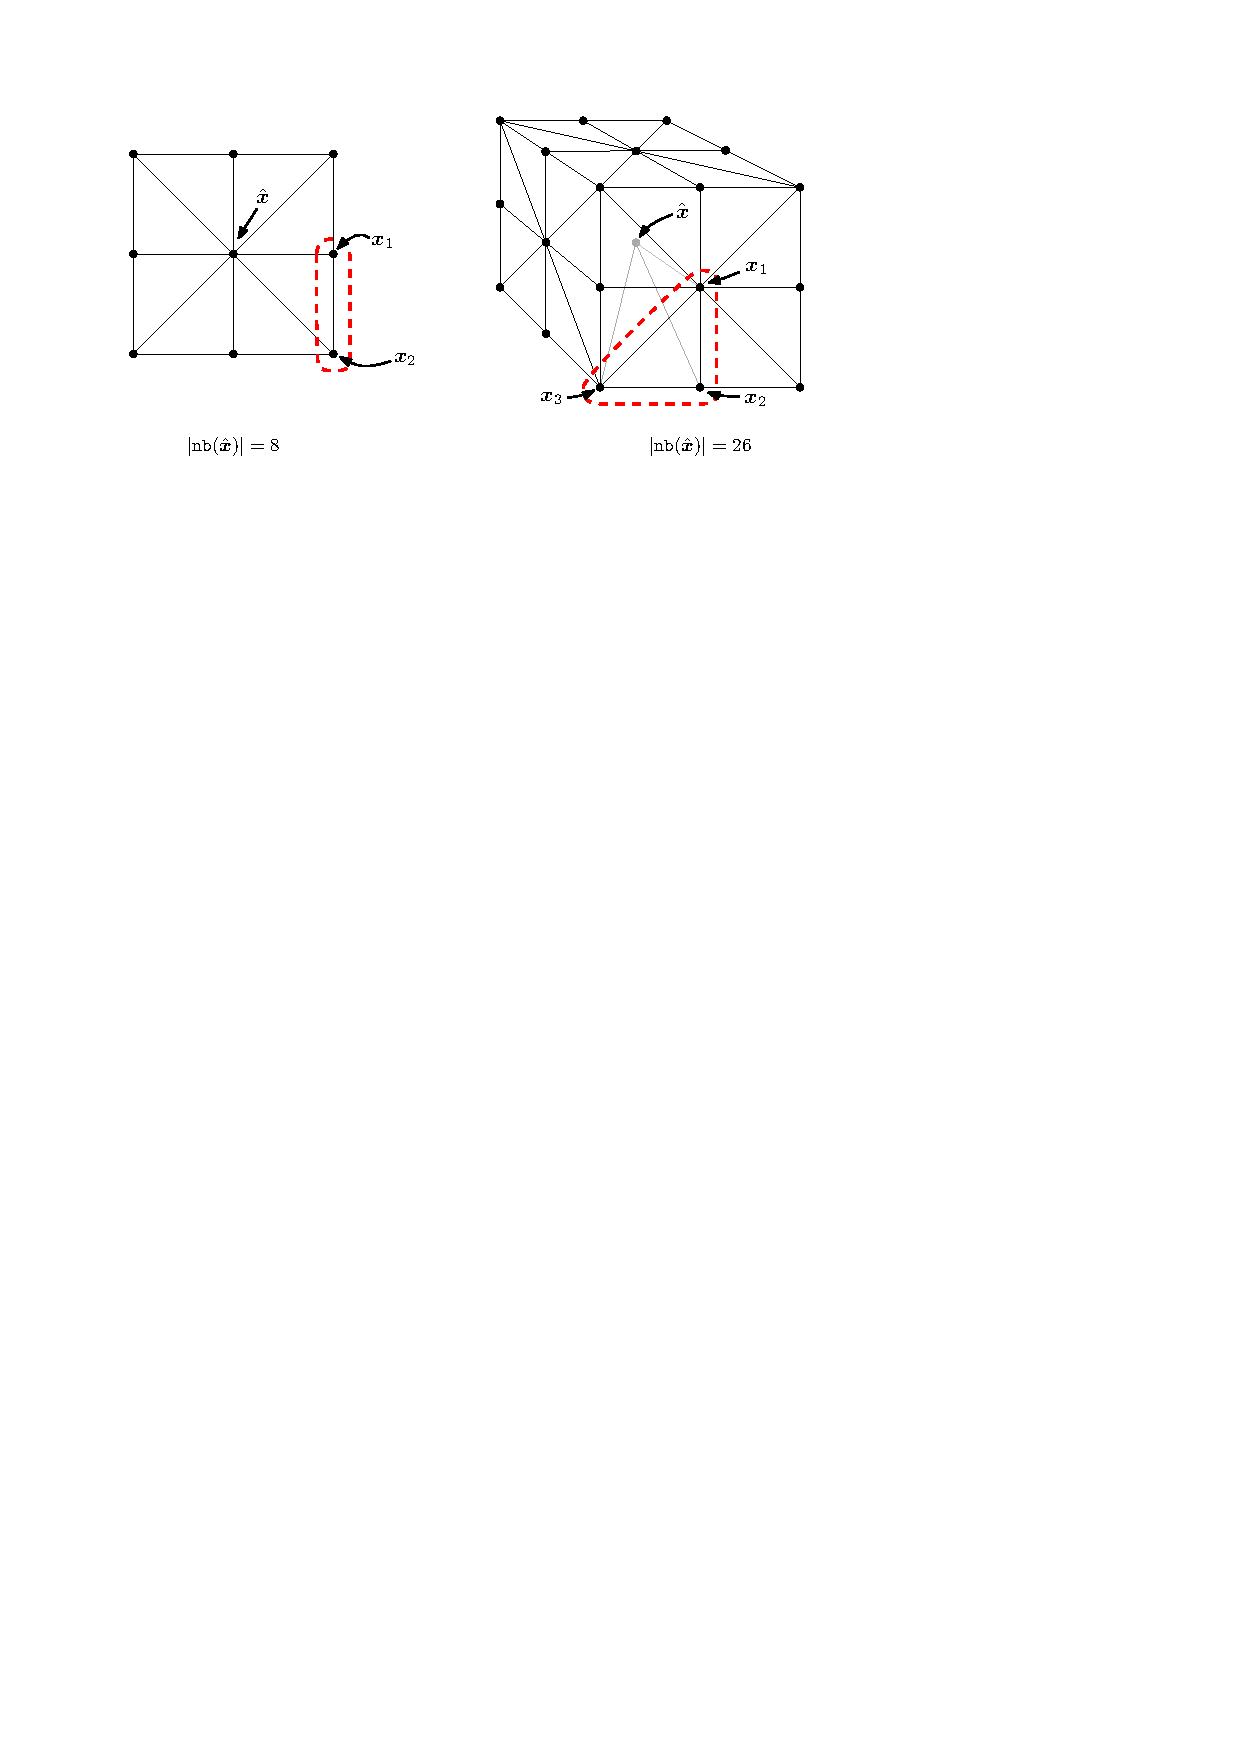
\includegraphics{neighborhoods.pdf}
%   \caption{\textbf{TODO}}\label{fig:neighborhoods}
% \end{figure}

To fix the idea in 3D, consider $\nb(\m{x})$ as shown in Figure\
\ref{fig:neighborhoods}, for which $|\nb(\m{x})| = 26$. There are 26
``line'' updates, where $d = 1$. To start with, each $\valid$ line
update is done, and $\m{x}_1$ for the minimizing line update is
recorded. Next, we fix $\m{x}_1$ and perform ``triangle'' updates
($d = 2$) where $\m{x}_2$ is varying. In this case, we can restrict
the number of triangle updates that are done by assuming either that
$(\m{x}_1, \m{x}_2)$ is an edge of mesh discretizing the surface of
the 3D stencil shown in Figure\ \ref{fig:neighborhoods}, or that
$\|\m{x}_1 - \m{x}_2\|$ is small enough (measuring the distance of
these two points in different norms leads to a different number of
triangle updates---we find the $\ell_1$ norm to work well). Finally,
we fix $\m{x}_2$ corresponding to the minimizing triangle update, and
do tetrahedron updates containing $\m{x}_1$ and $\m{x}_2$. Throughout
this process, $\m{x}_1, \m{x}_2$, and $\m{x}_3$ must all be $\valid$.

We emphasize that our work-efficient OLIM update algorithms work
equally well for the class of algorithms developed here. The main
differences between the JMMs studied here and the earlier OLIMs are
the cost functionals and the we way approximate $T$.

\section{Initialization methods}

A common problem with the convergence of numerical methods for solving
the eikonal equation concerns how to treat rarefaction fans. Our
numerical tests consist of point source problems, for which this
problem arises. A standard approach is to introduce the factored
eikonal equation~\cite{Fomel:2009aa}. If a point source is located at
$\m{x}^\circ \in \Omega_h$ and if we set $\Gamma_h = \{\m{x}^\circ\}$,
then we let $d(\m{x}) = \|\m{x} - \m{x}^\circ\|$ and use the ansatz:
\begin{equation}
  \tau(\m{x}) = z(\m{x}) + d(\m{x}), \qquad \m{x} \in \Omega.
\end{equation}
We insert this into the eikonal equation, modifying our numerical
methods as necessary, and solve for $z(\m{x})$ instead. This is not
complicated---see our previous work on OLIMs for solving the eikonal
equation to see how the cost functions should generally be
modified~\cite{Potter:2019ab,Yang:2019aa}.

It has been observed that only factoring the eikonal equation locally
gives the best results~\cite{Qi:2019aa}. In particular, for $\m{x}$
such that $d(\m{x}) < r^\circ$, where $r^\circ = O(1)$, we solve:
\begin{equation}
  \|\nabla z(\m{x}) + \nabla d(\m{x})\| = s(\m{x}),
\end{equation}
and the normal eikonal equation outside of this ball. We note that a
method for higher-order local factoring has been
developed~\cite{Luo:2014aa}. We leave combining this with our
algorithm for future work.

Yet another approach would be to solve the characteristic equations to
high-order for each $\m{x}$ in such a ball. This would require solving
$O(N)$ boundary value problems, each discretized into $O(N^{1/3})$
intervals, resulting in an $O(N^{4/3})$ cost overall (albeit with a
very small constant). One issue with this approach is that it only
works well if the ball surrounding $\m{x}^\circ$ is contained in the
interior of $\Omega$.

For our numerical experiments, we simply initialize $T$ and $\nabla T$
to the correct, ground truth values in a ball or box of constant size
centered at $\m{x}^\circ$.

\section{Cell marching}

Of particular interest is solving the transport equation governing $A$
while simultaneously solving the eikonal equation. Equation
\eqref{eq:transport-equation} can be solved using upwind finite
differences~\cite{Benamou:1996aa} or paraxial
raytracing~\cite{Popov:2002aa}. We prefer the latter approach since it
can be done locally, using the characteristic path $\mphi$ recovered
when computing $T(\xhat)$. Either approach requires accurate second
derivative information (we need $\Delta T$ for upwind finite
differences, or $\nabla^2 T$ for paraxial raytracing).

For the purposes of explanation and our numerical tests, we consider a
rectilinear grid with square cells in $\mathbb{R}^2$. On each cell,
our goal is to build a bicubic interpolant, approximating
$T(\m{x})$. This requires knowing $T, \nabla T$, and $T_{xy}$ at each
cell corner. If we know these values with $O(h^{4-p})$ accuracy, where
$p$ is the order of the derivative, then the bicubic is $O(h^{4-p})$
accurate over the cell. So far, we have described an algorithm that
marches $T$ and $\nabla T$, which are sometimes termed the \emph{total
  1-jet}. We now show how $T_{xy}$ can also be marched, allowing us to
march the \emph{partial 1-jet}.\footnote{The total $k$-jet of a
  function $f$ is the set $\{\partial^{\m{\alpha}}f\}_{\m{\alpha}}$,
  where $\|\m{\alpha}\|_1 \leq k$; the partial $k$-jet is
  $\{\partial^{\m{\alpha}} f\}_{\m{\alpha}}$ where
  $\|\m{\alpha}\|_\infty \leq k$.}

\begin{figure}
  \centering
  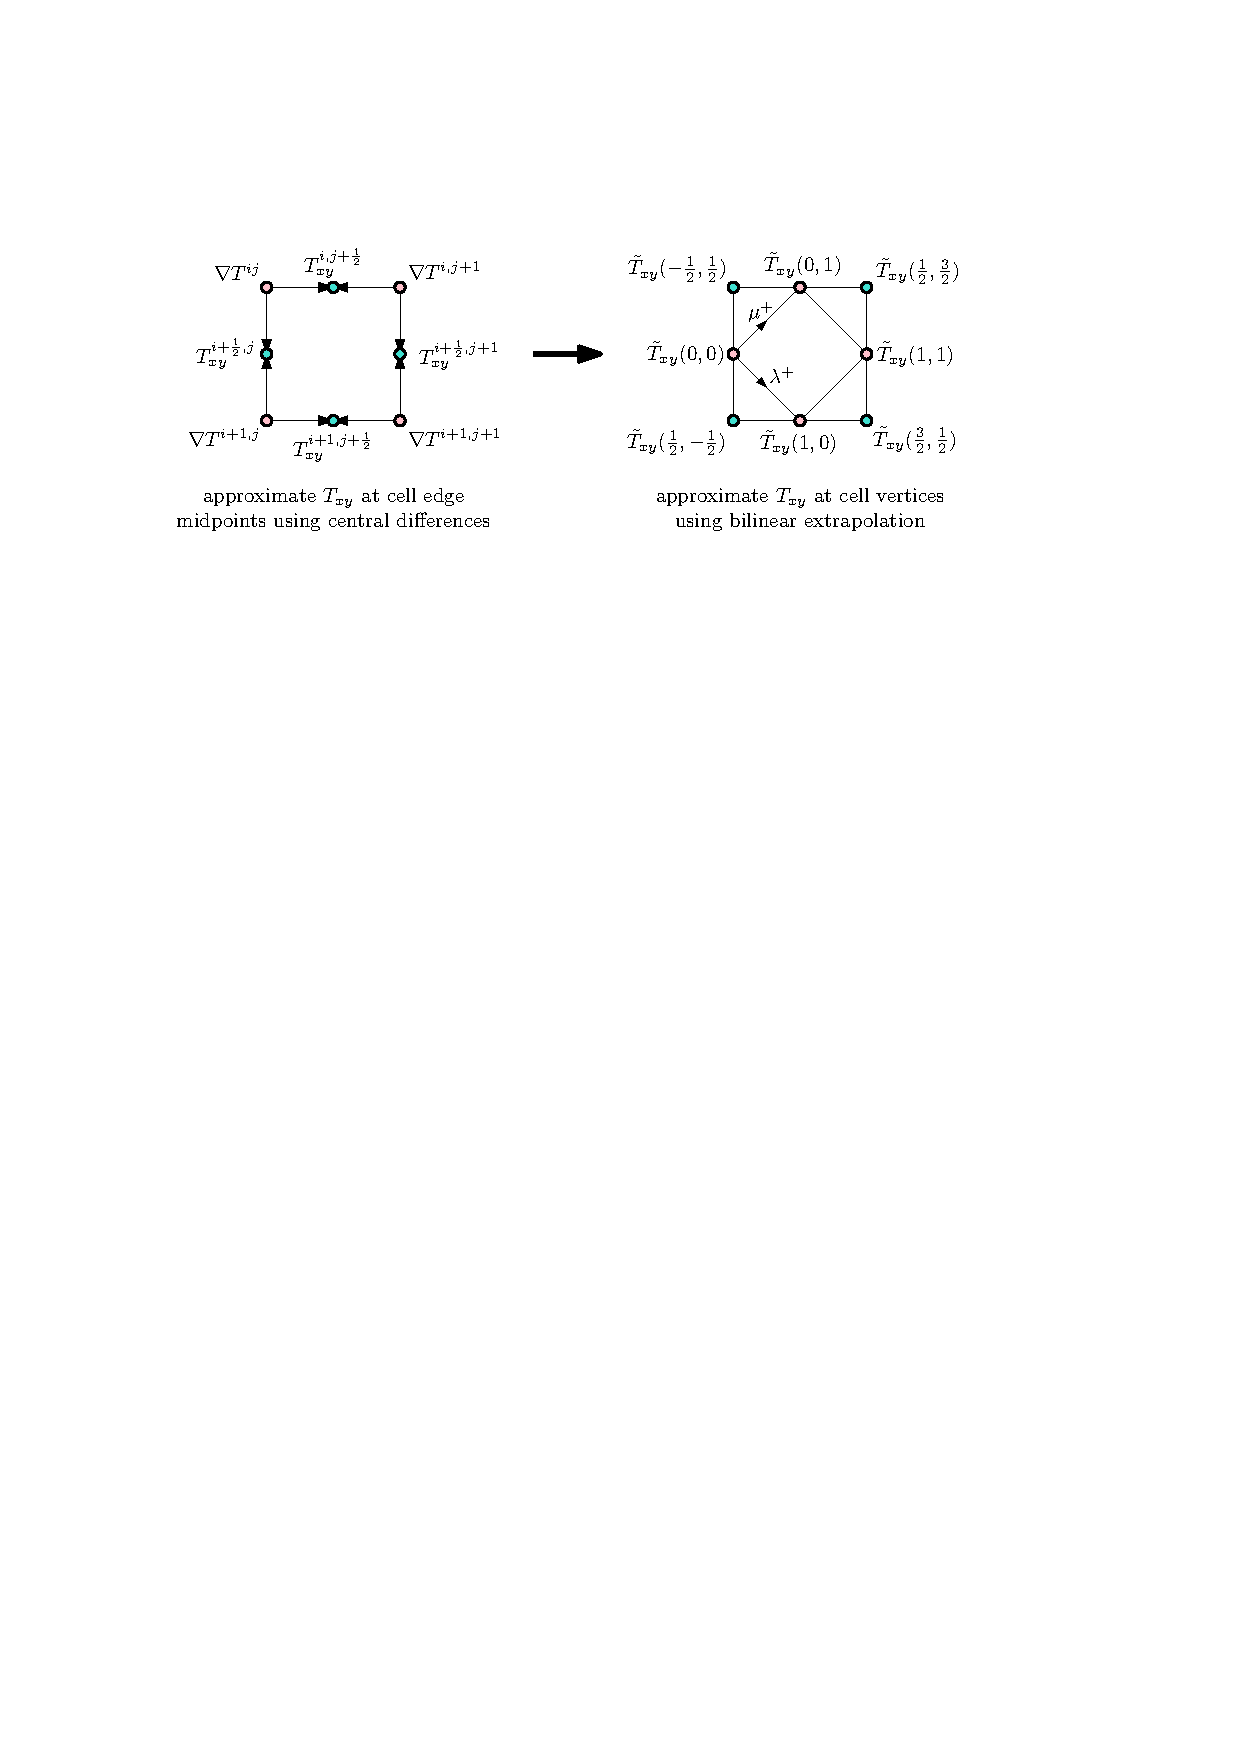
\includegraphics[width=\textwidth]{estimate-Txy.pdf}
  \caption{\emph{Cell-based interpolation.} To approximate the mixed
    second partials of a function with $O(h^2)$ accuracy from $O(h^3)$
    accurate gradient values available at the corners of a cell, the
    following method of using central differences to approximate the
    mixed partials at the midpoints of the edges of the cell, followed
    by bilinear extrapolation, can be used.}\label{fig:estimate-Txy}
\end{figure}

Let $\m{x}_{ij}$ with $(i, j) \in \{0, 1\}^2$ denote the corners of a
square cell with sides of length $h$, and assume that we know
$\nabla T(\m{x}_{ij})$ with $O(h^3)$ accuracy. We can use the
following approach to estimate $T_{xy}(\m{x}_{ij})$ at each corner:
\begin{itemize}
\item First, at the midpoints of the edges oriented in the $x$
  direction (resp., $y$ direction), approximate $T_{xy}$ using the
  central differences involving $T_y$ (resp., $T_x$) at the
  endpoints. This approximation is $O(h^2)$ accurate at the midpoints.
\item Use bilinear extrapolation to reevaluate $T_{xy}$ at the corners
  of the cell, yielding $T_{xy}(\m{x}_{ij})$, also with $O(h^2)$
  accuracy.
\end{itemize}
This procedure is illustrated in Figure\ \ref{fig:estimate-Txy}.

\begin{figure}
  \centering
  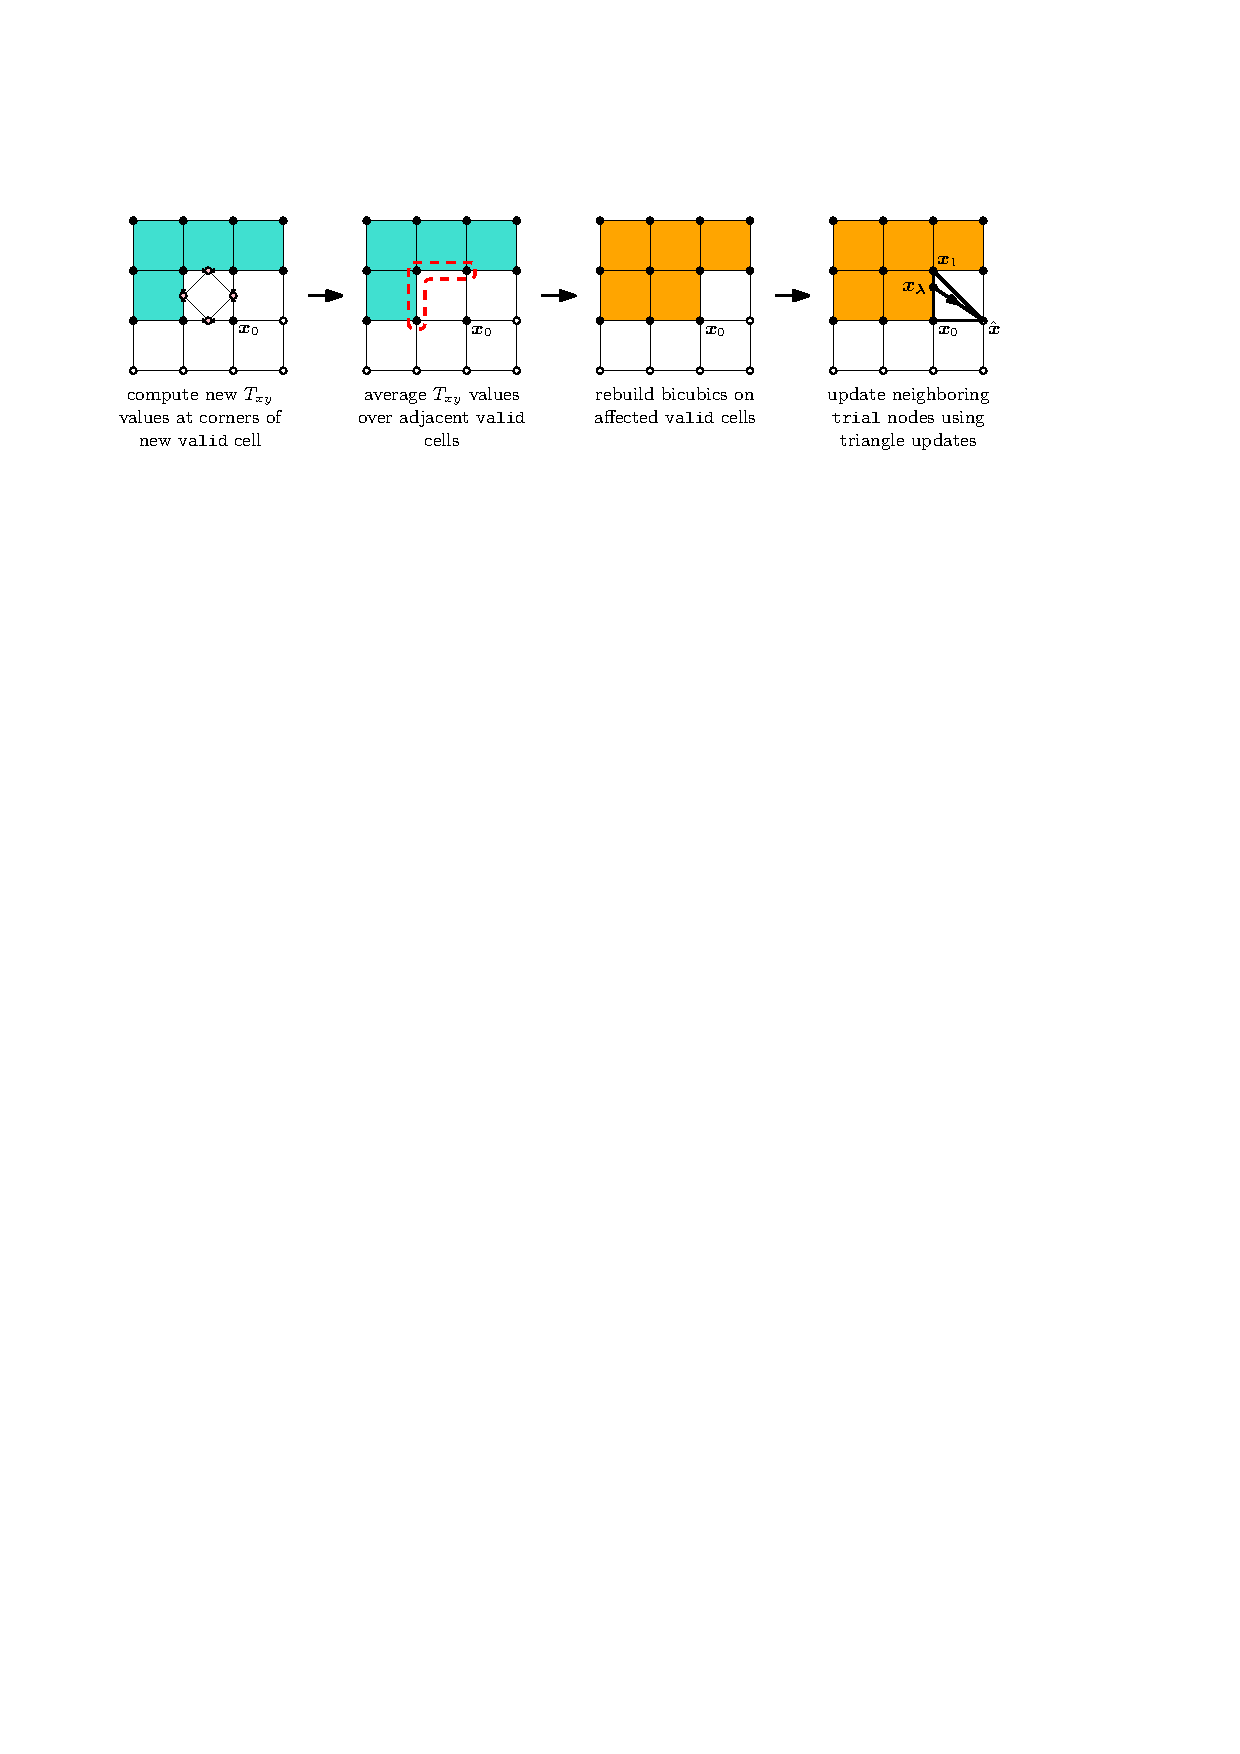
\includegraphics[width=\linewidth]{rebuild-cells.pdf}
  \caption{\emph{Local cell marching.} After computing values of
    $T_{xy}$ as shown in Figure~\ref{fig:estimate-Txy} (\emph{left}),
    to ensure continuity of the global interpolant, nodal values
    incident on the newly \texttt{valid} cell (containing $x_0$) can
    be recomputed by averaging over $T_{xy}$ values taken from
    incident \texttt{valid} cells (\emph{middle}). Finally, a bicubic
    cell-based interpolant is constructed
    (\emph{right}).}\label{fig:rebuild-cells}
\end{figure}

One issue with this approach is that it results in a piecewise
interpolant that is only $C^1$ globally. That is, if we estimate the
value of $T_{xy}$ at a corner from each of the cells which are
incident upon it, we will get different values in general. To compute
a globally $C^2$ piecewise interpolant, we can average $T_{xy}$ values
over incident $\valid$ cells, where we define a $\valid$ cell to be a
cell whose vertices are all $\valid$. How to do this is shown in
Figure\ \ref{fig:rebuild-cells}.

The idea of approximating the partial 1-jet from the total 1-jet in an
optimally local fashion by combining central differences with bilinear
extrapolation, and averaging nodal values over adjacent cells to
increase the degree of continuity of the interpolant, is borrowed from
Seibold et al.~\cite{Seibold:2011aa}. However, applying this idea in
this context, and doing the averaging in an upwind fashion is novel

The scheme arrived at in this way is no longer optimally
local. However, the sequence of operations described here can be done
on an unstructured triangle or tetrahedron mesh. This makes this
approach suitable for use with an unstructured mesh that conforms to a
complicated boundary.

We should mention here that our approach to estimating $T_{xy}$ is
referred to as \emph{twist estimation} in the \emph{computer-aided
  design} (CAD) community~\cite{Farin:2014aa}, where other approaches
have been proposed~\cite{Brunet:1985aa,Hagen:1987aa}. We leave the
adaptation of these ideas to the present context for future work.

\section{Numerical experiments} In this section, we first present a
variety of test problems which differ primarily in the choice of
slowness function $s$. The choices of $s$ range from the simple, such
as $s \equiv 1$ (a reasonable first choice for speed of sound in room
acoustics), to more strongly varying. We then present experimental
results for our different JMMs as applied to these different slowness
functions, demonstrating the significant effect the choice of $s$ has
on solver accuracy. We note that $s$ does not significantly affect the
runtime of any of our solvers---our solvers run in
$O(|\Omega_h| \log |\Omega_h|)$ time, where the constant factors are
essentially insensitive to the choice of $s$.

\subsection{Test problems} Before presenting our experimental results,
we collect the details of each problem setup. These test problems
primarily differ by the choice of $s$. We generally consider point
source problems on $\Omega = [-1, 1] \times [-1, 1]$. In some cases,
we use $\Omega = [0, 1] \times [0, 1]$, due to the behavior of the
characteristics of $\tau$ (i.e., some choices of $s$ result in shadow
zones that are unreachable by rays).

\paragraph{Constant slowness with a point source} For this problem, the slowness and solution are given by:
\begin{equation}
  s \equiv 1, \qquad \tau(\m{x}) = \|\m{x}\|.
\end{equation}
We take the domain to be
$\Omega = [-1, 1] \times [-1, 1] \subseteq \mathbb{R}^2$. To control
the size of the discretized domain, we let $M > 0$ be an integer and
set $h = 1/M$, from which we define $\Omega_h$ accordingly. We place a
point source at $\m{x}^\circ = (0, 0) \in \Omega_h$. The set of
initial boundary data locations given by is
$\Gamma_h = \{\m{x}^\circ\}$, with boundary conditions given by
$g(\m{x}^\circ) = 0$.

\paragraph{Linear speed with a point source (\#1)} Our next test
problem has a linear velocity profile. This might model the variation
in the speed of sound due to a linear temperature gradient (e.g., in a
large room). The slowness is given by:
\begin{equation}
  s(\m{x}) = \left[\frac{1}{s_0} + \m{v}^\top \m{x}\right]^{-1},
\end{equation}
where $s_0 > 0$, and $\m{v} \in \mathbb{R}^2$ are parameters. The
solution is given by:
\begin{equation}\label{eq:eikonal-linear-speed}
  \tau(\m{x}) = \frac{1}{\|\m{v}\|} \cosh^{-1}\hspace{-0.1em}\left(1 + \frac{1}{2} s_0 s(\m{x}) \|\m{v}\|^2 \|\m{x}\|^2\right).
\end{equation}
For our first test with a linear speed function, we take $s_0 = 1$ and
$\m{v} = (0.133, -0.0933)$. The domain, discretized domain, and
boundary data are the same as for the constant slowness point source
problem described previously.

\paragraph{Linear speed with a point source (\#2)} For our second
linear speed test problem, we set $s_0 = 2$ and $\m{v} = (0.5,
0)$. For this problem, we let $\Omega = [0, 1] \times [0, 1]$,
discretize into $M$ nodes along each axis, and define $\Omega_h$
accordingly (i.e., $|\Omega_h| = M^2$, with $M = h^{-1}$). We take
$\m{x}^\circ$, $\Gamma_h$, and $g$ to be same as in the previous two
test problems.

\paragraph{A nonlinear slowness function involving a sine function}
For $\m{x} = (x_1, x_2)$, we set:
\begin{equation}
  \tau(\m{x}) = \frac{x_1^2}{2} + 2 \sin\hspace{-0.1em}\left(\frac{x_1 + x_2}{2}\right)^2.
\end{equation}
This eikonal has a unique minimum, $\tau(0, 0) = 0$, and is strictly
convex in $\Omega = [-1, 1]^2$. This lets us determine the slowness
from the eikonal equation, giving:
\begin{equation}
  s(\m{x}) = \sqrt{\sin(x_1 + x_2)^2 + \big(x_1 + \sin(x_1 + x_2)\big)^2}.
\end{equation}
For this test problem, we take $\Gamma_h$ and $\Omega_h$ as in the
constant slowness point source problem.

\paragraph{Sloth} \textbf{TODO}: \emph{finishing adding explanation.}

\begin{equation}
  s(\m{x}) = \sqrt{s_0^2 + \m{v}^\top \m{x}}.
\end{equation}
For our test with this slowness function, we set $s_0 = 2$, and
$\m{v} = (0, -3)$. In this case, to avoid caustics, we take
$\Omega = [0, \tfrac{1}{2}]^2$. The discretized domain and boundary
data are determined analogously to the earlier cases.

\subsection{Experimental results}

\begin{figure}
  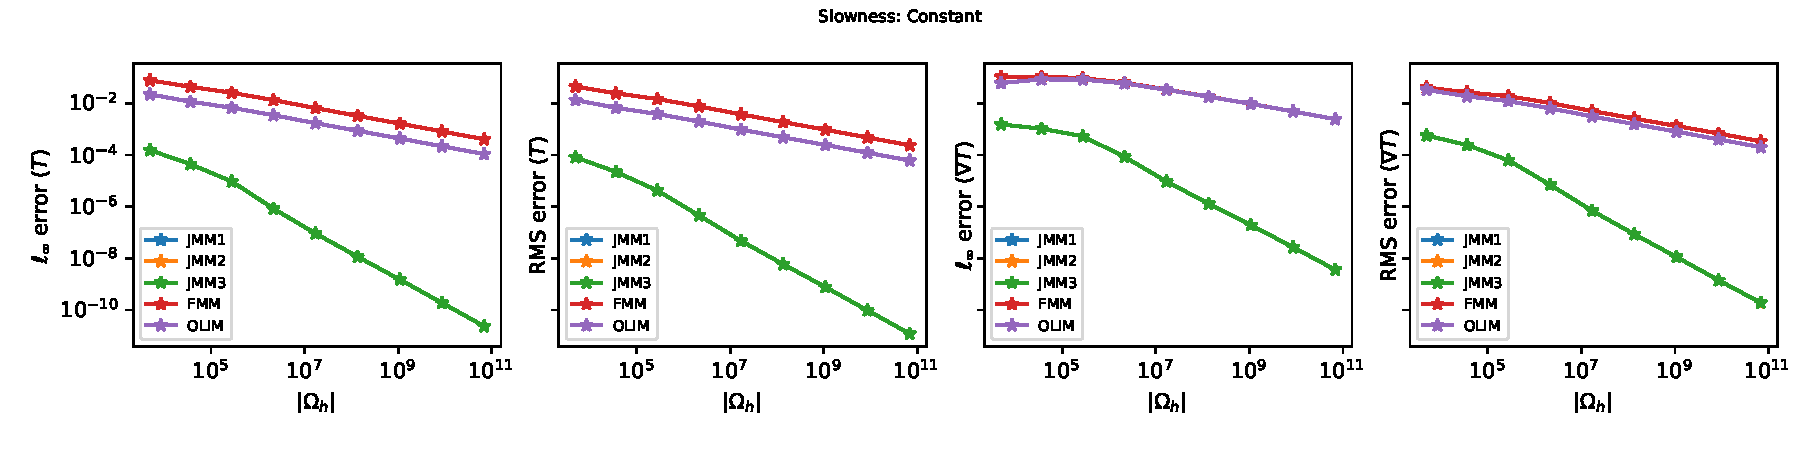
\includegraphics[width=\textwidth]{plots/size_vs_errors_1.pdf}
  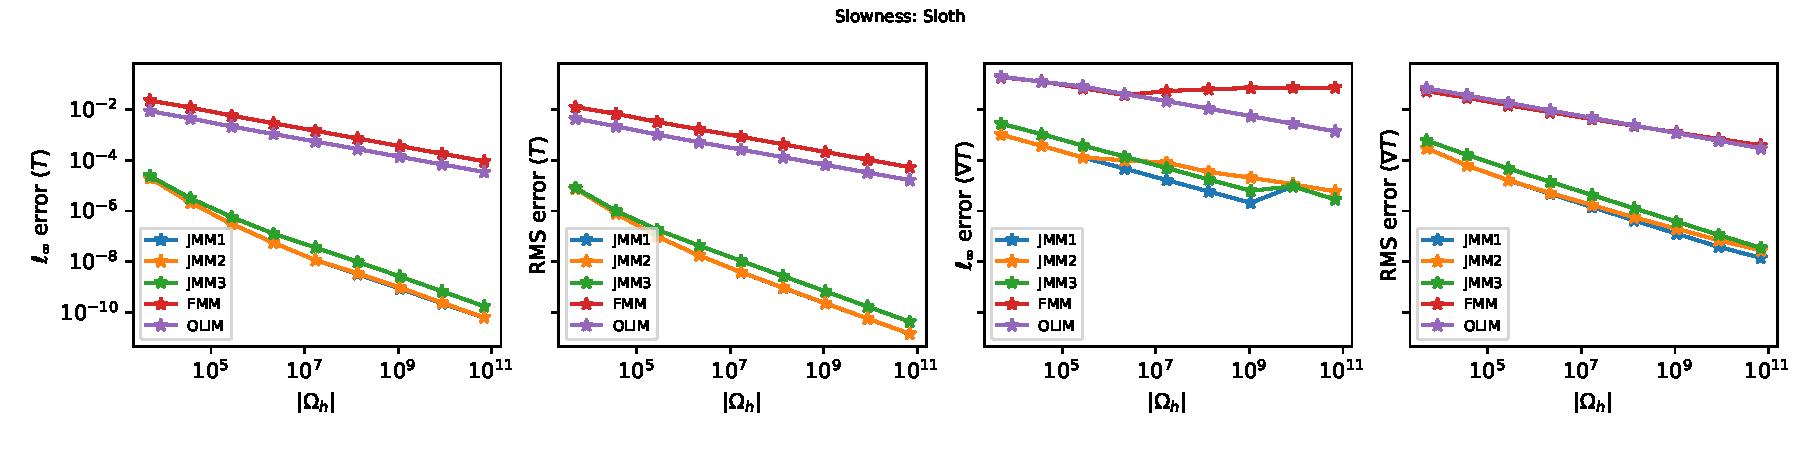
\includegraphics[width=\textwidth]{plots/size_vs_errors_g.pdf}
  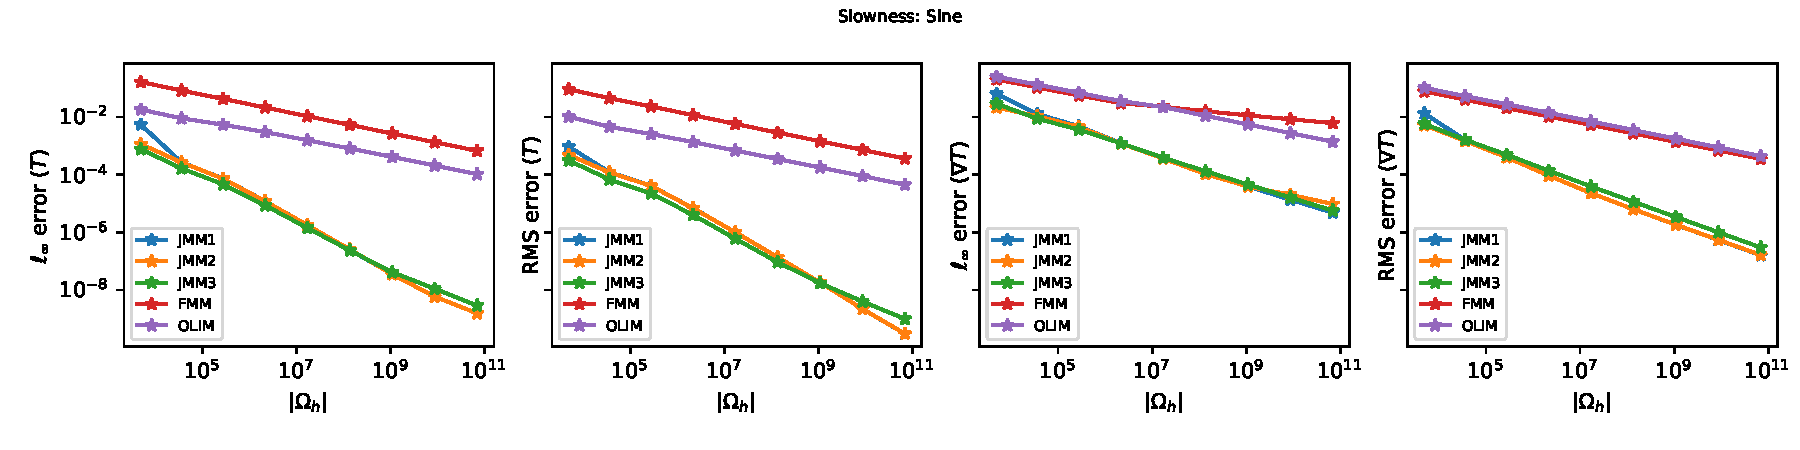
\includegraphics[width=\textwidth]{plots/size_vs_errors_m.pdf}
  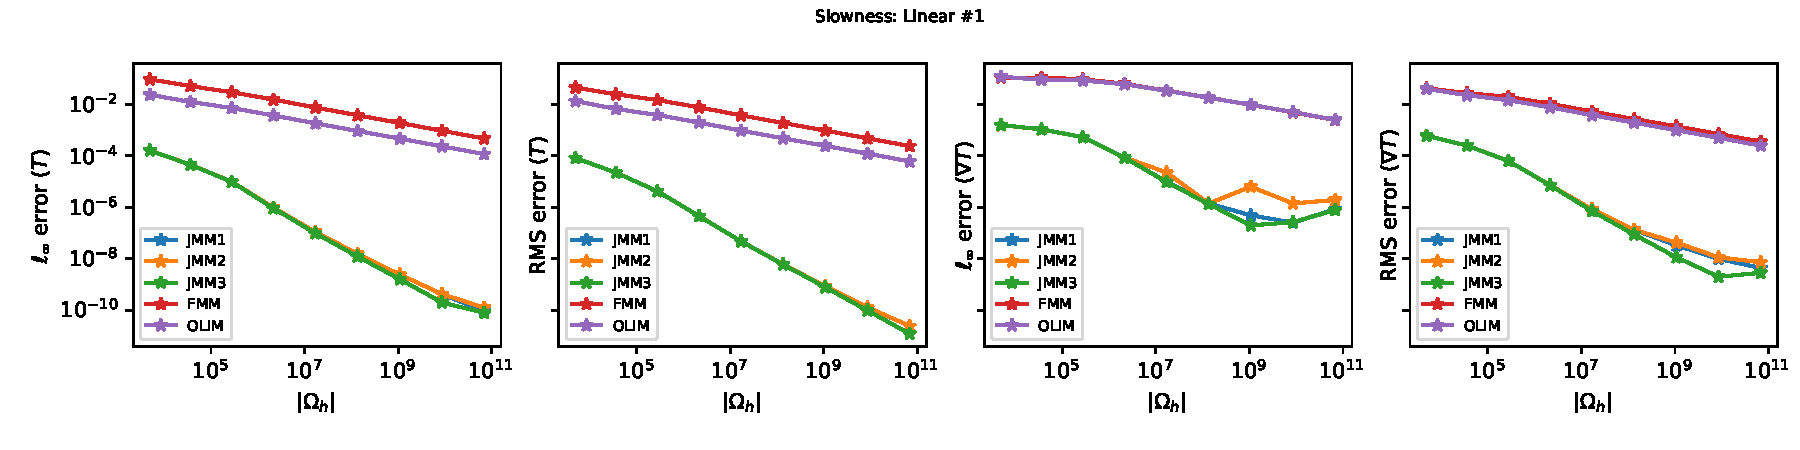
\includegraphics[width=\textwidth]{plots/size_vs_errors_p.pdf}
  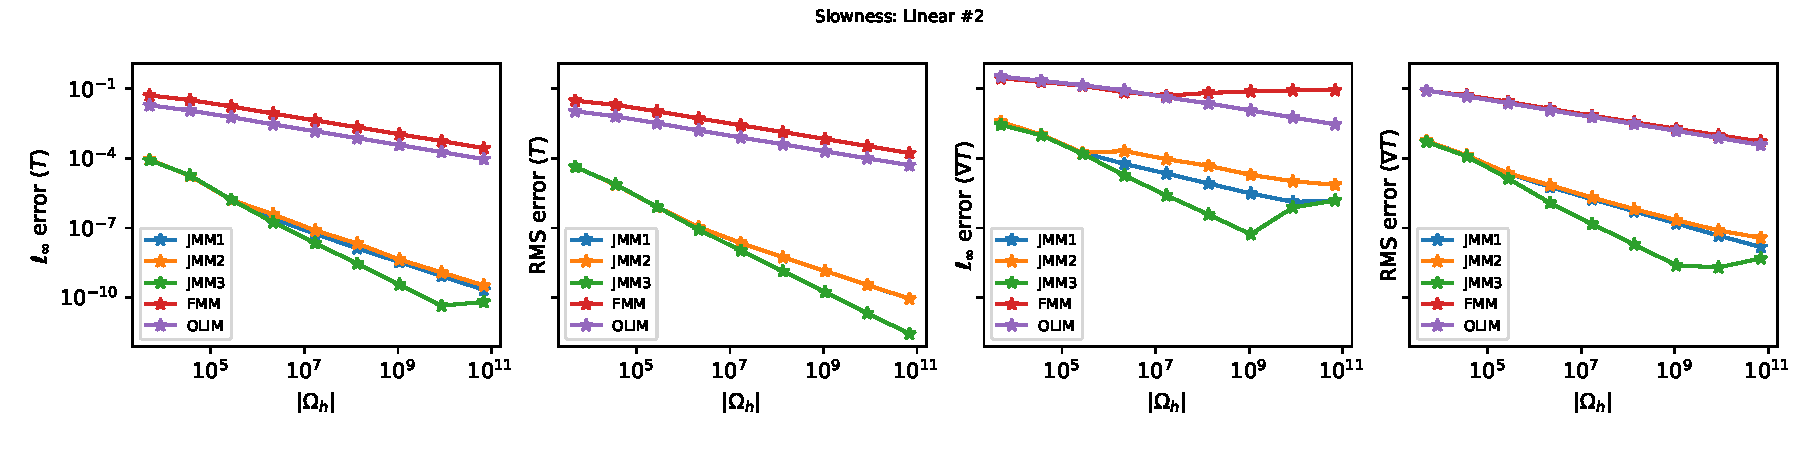
\includegraphics[width=\textwidth]{plots/size_vs_errors_v.pdf}
  \caption{Plots comparing domain size ($|\Omega_h|$) and
    errors.}\label{fig:size-vs-error}
\end{figure}

\begin{figure}
  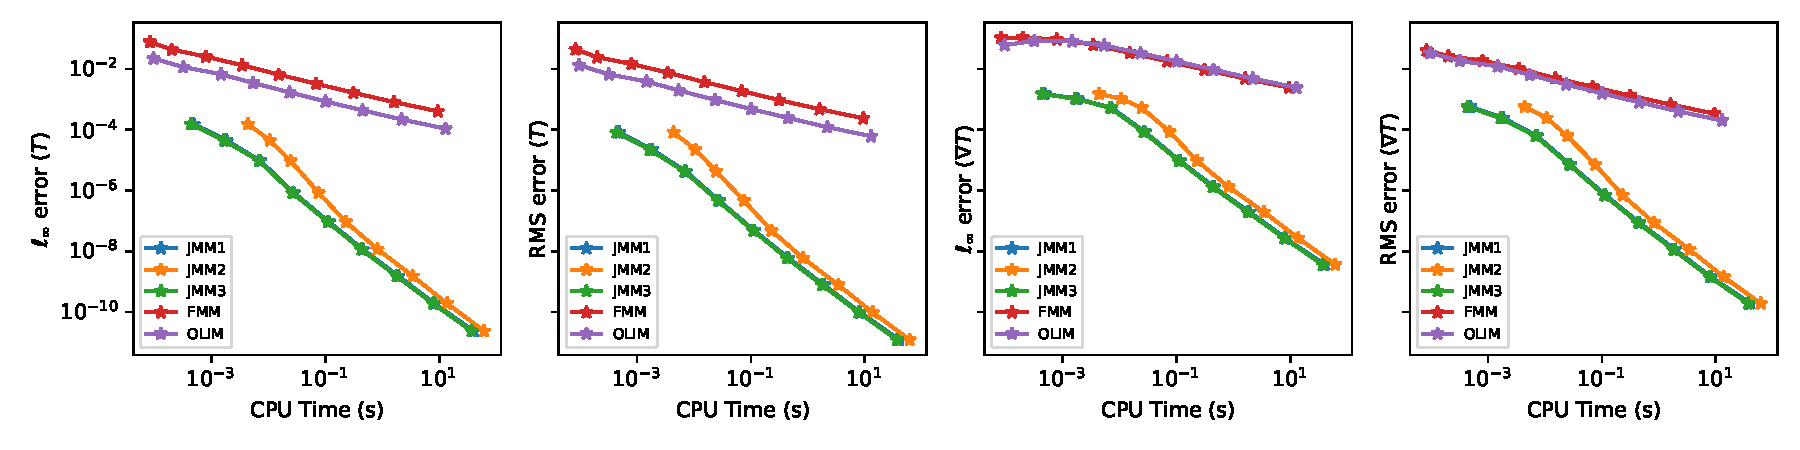
\includegraphics[width=\textwidth]{plots/time_vs_errors_1.pdf}
  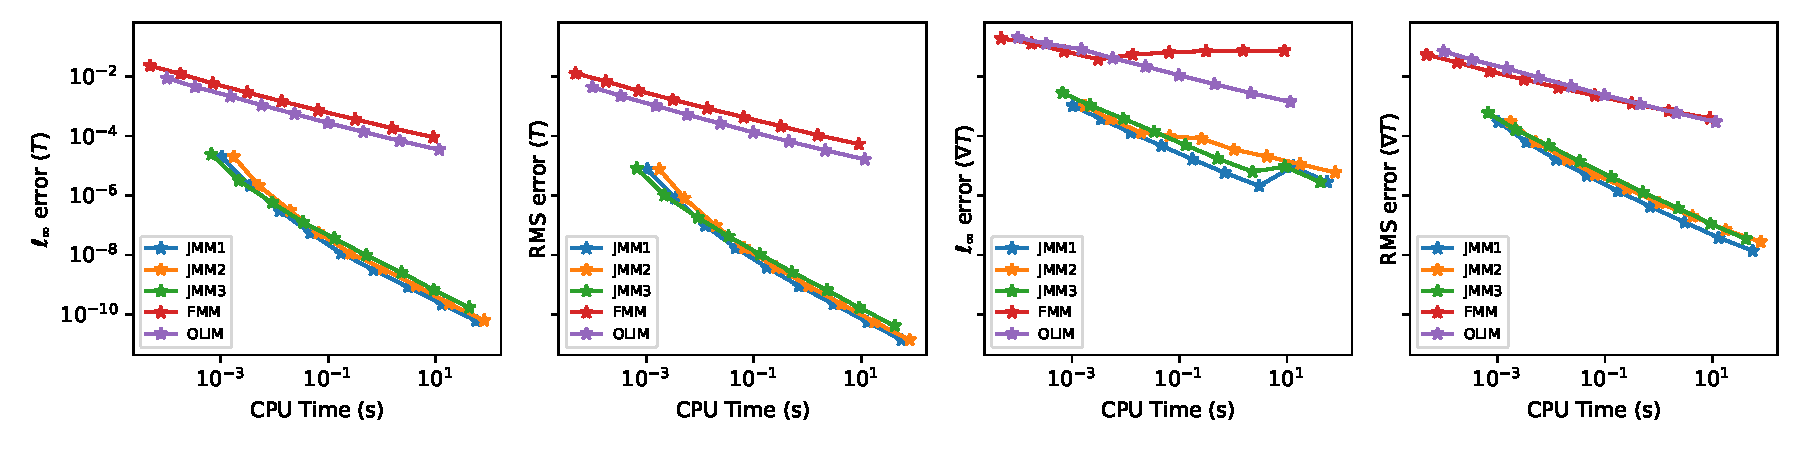
\includegraphics[width=\textwidth]{plots/time_vs_errors_g.pdf}
  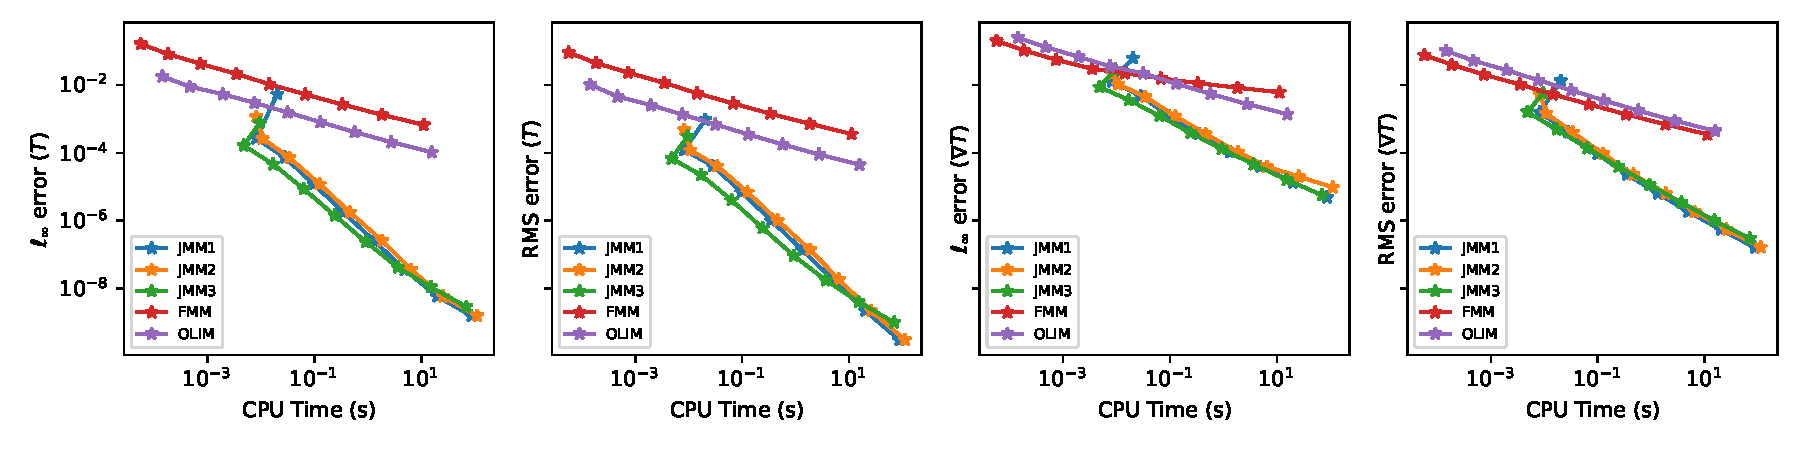
\includegraphics[width=\textwidth]{plots/time_vs_errors_m.pdf}
  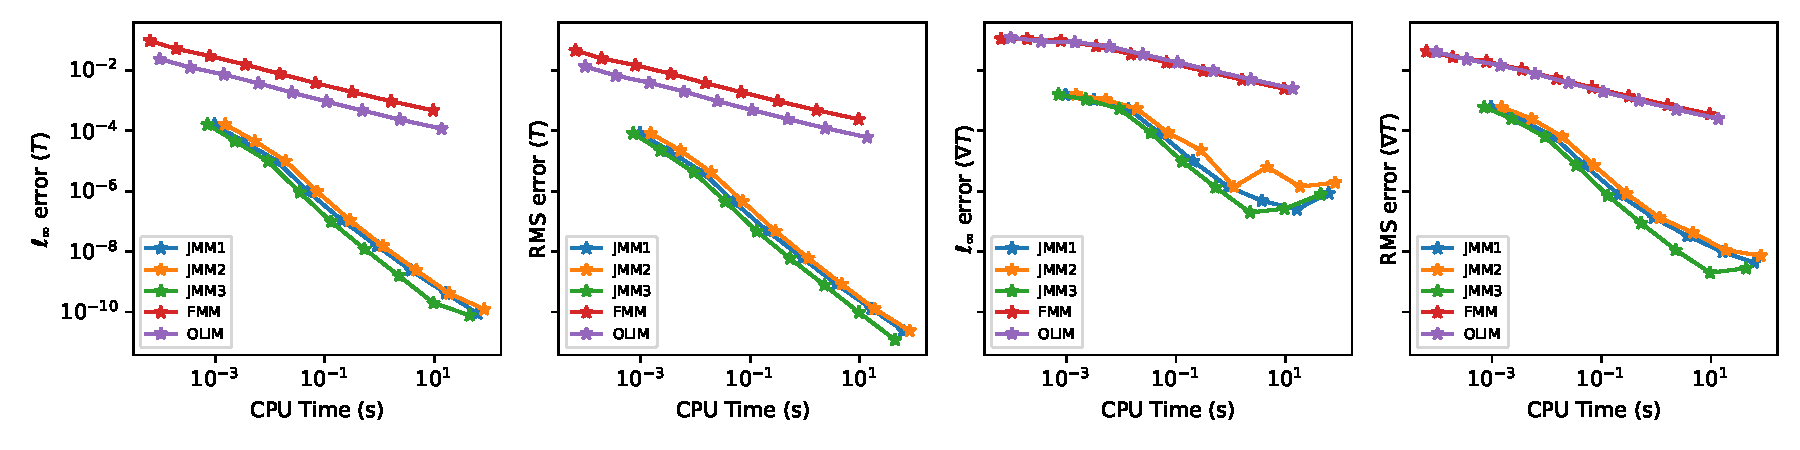
\includegraphics[width=\textwidth]{plots/time_vs_errors_p.pdf}
  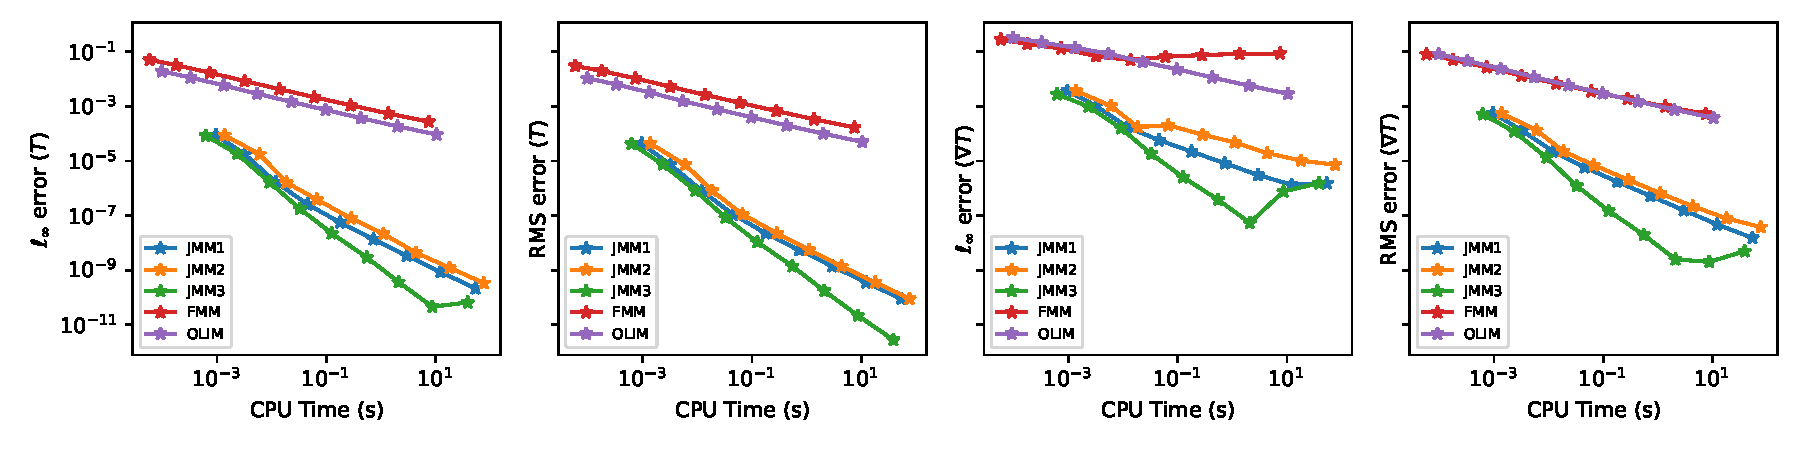
\includegraphics[width=\textwidth]{plots/time_vs_errors_v.pdf}
  \caption{Plots comparing CPU runtime in seconds and
    errors.}\label{fig:time-vs-error}
\end{figure}

\begin{table}
  \centering
  \begin{tabular}{cccccc}
    & JMM & $E_{\mbox{max}} (T)$ & $E_{\mbox{RMS}} (T)$& $E_{\mbox{max}} (\nabla T)$ & $E_{\mbox{RMS}} (\nabla T)$ \\
    \midrule
    \multirow{3}{*}{Constant}
    & \#1 & 2.92 & 2.92 & 2.49 & 2.82 \\
    & \#2 & 2.92 & 2.92 & 2.49 & 2.82 \\
    & \#3 & 2.92 & 2.92 & 2.49 & 2.82 \\
    \midrule
    \multirow{3}{*}{Linear \#1}
    & \#1 & 2.72 & 2.83 & 1.76 & 2.33 \\
    & \#2 & 2.69 & 2.83 & 1.43 & 2.26 \\
    & \#3 & 2.81 & 2.92 & 1.81 & 2.55 \\
    \midrule
    \multirow{3}{*}{Linear \#2}
    & \#1 & 2.33 & 2.35 & 1.47 & 1.88 \\
    & \#2 & 2.24 & 2.35 & 1.07 & 1.74 \\
    & \#3 & 2.79 & 3.02 & 1.72 & 2.42 \\
    \midrule
    \multirow{3}{*}{Sine}
    & \#1 & 2.68 & 2.69 & 1.70 & 1.99 \\
    & \#2 & 2.53 & 2.63 & 1.48 & 1.89 \\
    & \#3 & 2.32 & 2.36 & 1.54 & 1.78 \\
    \midrule
    \multirow{3}{*}{Sloth}
    & \#1 & 2.23 & 2.32 & 1.08 & 1.78 \\
    & \#2 & 2.22 & 2.32 & 0.86 & 1.65 \\
    & \#3 & 2.07 & 2.13 & 1.25 & 1.75 \\
  \end{tabular}
  \caption{The order of convergence $p$ for each combination of test
    problems and solvers, computed for different types of errors and
    fit as $C h^p$.}\label{fig:least-squares-fits}
\end{table}

\textbf{TODO}: \emph{add discussion}

\section{Theoretical results} In this section we present two
theoretical results of interest:
\begin{itemize}
\item We prove consistency for the JMM presented in
  \ref{ssec:quadratic}. This results suggests that $O(h^2)$-accurate
  values of $T$ and $O(h)$ accurate $\nabla T$ values are to be
  expected in general, with certain choices of $s$ giving rise to
  $O(h^3)$ values of $T$ and $O(h^2)$, or even $O(h^3)$, values of
  $\nabla T$.
\item We demonstrate a counterexample that shows how using a 4-point
  stencil can degrade the overall order of convergence of a jet
  marching method, and how the use of an 8-point stencil overcomes
  this problem.
\end{itemize}

\subsection{Consistency of the quadratic curve JMM}

As we have seen, our numerical results indicate that we can expect
between $O(h^2)$ and $O(h^3)$ accuracy for $T(\m{x})$ and between
$O(h)$ and $O(h^2)$ accuracy for $\nabla T(\m{x})$. Our goal is to
determine the conditions under which $O(h^3)$-accurate $T$ and
$O(h^2)$-accurate $\nabla T$ obtains. Establishing theoretical lower
bounds on the order of convergence for $T$ and $\nabla T$ requires
tedious calculations and nuanced considerations, making the numerical
analysis of this solver an interesting and challenging problem in its
own right. We defer an extensive study of this problem to future
work. Here, we simply present consistency results for the simplified
JMM described in section~\ref{ssec:quadratic} for the case
$\Omega \subseteq \mathbb{R}^2$.

\begin{theorem}
  Let $\Omega \subseteq \mathbb{R}^2$, assume that
  $s \in C^2(\Omega)$, and let $(\xhat, \m{x}_1, \m{x}_2)$ be an
  update triangle where $\state(\xhat) = \trial$,
  $\state(\m{x}_1) = \valid$, and $\state(\m{x}_2) = \valid$. Assume
  that no caustic is incident on the update triangle, and that the ray
  arriving at $\xhat$ crosses the segment $[\m{x}_1, \m{x}_2]$. Then:
  \begin{equation}
    |\tau(\xhat) - T(\xhat)| = O(h^4), \qquad \|\nabla \tau(\xhat) - \nabla T(\xhat)\| = O(h^2).
  \end{equation}
\end{theorem}

\begin{proof}
  A detailed proof this theorem requires lengthy but straightforward
  calculations, and will be presented elsewhere; so, instead, we give
  an outline of the proof.

  Let $\m{x}_{\lambda} = (1 - \lambda) \m{x}_1 + \lambda + \m{x}_2$,
  we define:
  \begin{equation}\label{eq:exact-functional-with-chordal-parametrization}
    f(\lambda) = \tau(\m{x}_{\lambda}) + \int_0^{L_\lambda} s(\mphi(\sigma)) \|\mphi'(\sigma)\| d\sigma,
  \end{equation}
  where $L_\lambda = \|\xhat - \m{x}_\lambda\|$, and let
  $F(\m{x}_{\lambda}, \m{t})$ be the cost functional given
  by~\eqref{eq:quadratic-cost-functional}. Here, we parametrize the
  line integral
  in~\eqref{eq:exact-functional-with-chordal-parametrization} using a
  chordal parametrization. Note that:
  \begin{equation}
    \tau(\xhat) = \min_{0 \leq \lambda \leq 1} f(\lambda), \qquad T(\xhat) = \min_{0 \leq \lambda \leq 1} F(\m{x}_\lambda, \m{t}(\m{x}_\lambda)),
  \end{equation}
  and that the  gradients can recovered via:
  \begin{equation}
    \nabla \tau(\xhat) = s(\xhat) \frac{\mphi'(L_\lambda)}{\|\mphi'(L_\lambda)\|}, \qquad \nabla T(\xhat) = s(\xhat) \m{t}(\m{x}_\lambda).
  \end{equation}
  From these expressions, using multivariable calculus and classical
  interpolation theory~\cite{Stoer:2013aa}, we show that:
  \begin{equation}
    |f(\lambda) - F(\lambda)| \leq Ch^4, \qquad 0 \leq h \leq 1,
  \end{equation}
  where $C > 0$ is a constant. Then, using this fact, we can show:
  \begin{equation}
    \left|\min_{0\leq\lambda\leq1} f(\lambda) - \min_{0\leq\lambda\leq1} F(\lambda)\right| \leq Ch^4.
  \end{equation}
  This establishes that $|\tau(\xhat) - T(\xhat)| = O(h^4)$. To bound
  the error in the gradients, we first show that
  $|f'(\lambda) - F'(\lambda)| = O(h^3)$. Then, we prove that:
  \begin{equation}
    F''(\lambda) \geq C'h, \qquad 0 \leq \lambda \leq 1,
  \end{equation}
  where $C' > 0$ is another positive constant. It follows from the
  intermediate value theorem that:
  \begin{equation}
    \left|\Arg\min_{0\leq\lambda\leq1}f(\lambda) - \Arg\min_{0\leq\lambda\leq1}F(\lambda)\right| = O(h^2),
  \end{equation}
  which we use to establish
  $\|\nabla \tau(\xhat) - \nabla T(\xhat)\| = O(h^2)$.
\end{proof}

\subsection{A counterexample that demonstrates the need for the
  8-point stencil}\label{ssec:counterexample}

\begin{figure}
  \centering
  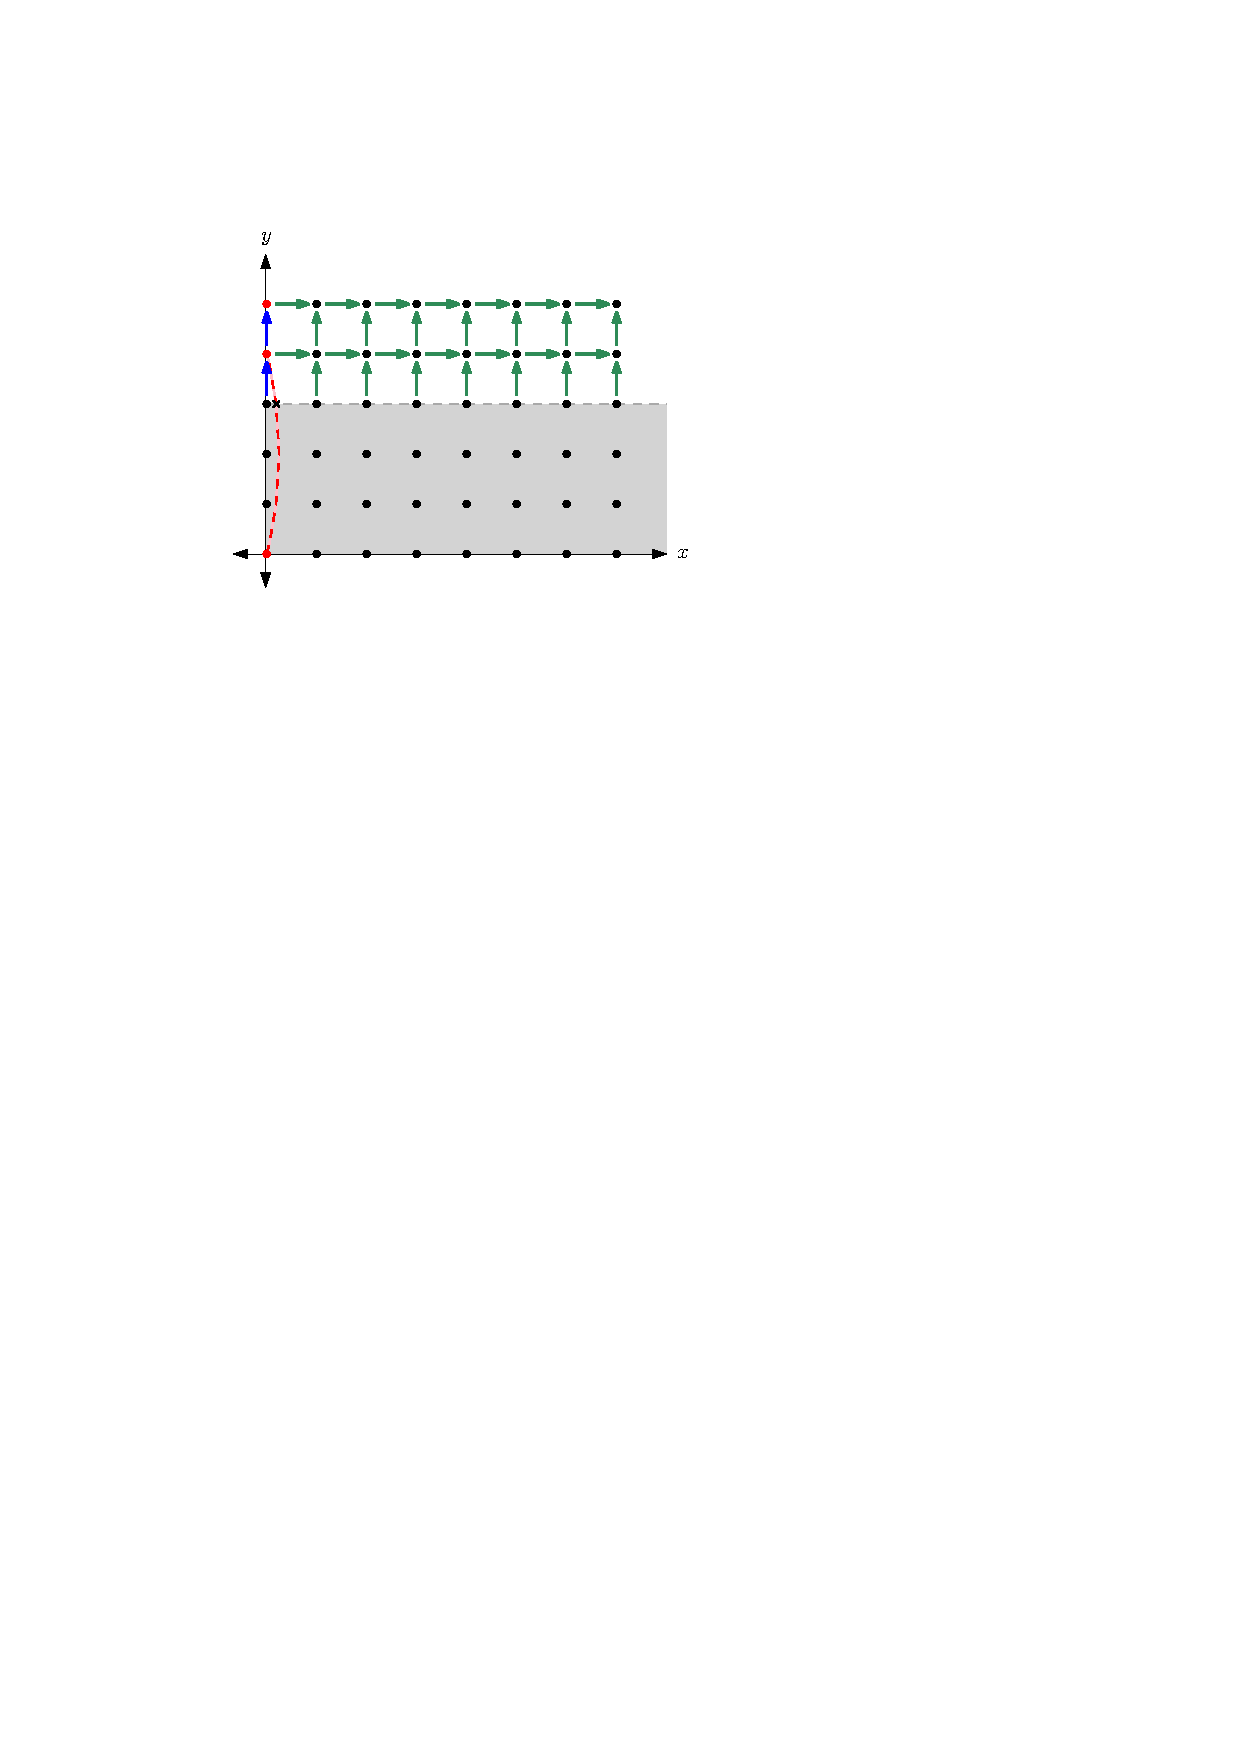
\includegraphics{bad-4point.pdf}
  \caption{\textbf{TODO}}
\end{figure}

On a regular grid in $\mathbb{R}^2$, first-order eikonal solvers that
use either a 4-point or 8-point stencil are known to work
reliably. The use of an 8-point stencil typically improves the error
constant by an order of magnitude; in $\mathbb{R}^3$, the differences
between the 6-point and 26-point stencils are roughly the
same~\cite{Potter:2019ab}. We are not aware of any thorough studies of
the effect of stencils on higher-order solvers.

In this section, we provide a counterexample that demonstrates that
using the 4-point stencil can limit the rate of convergence of a JMM
to quadratic. Consider the following linear speed function:
\begin{equation}
  s : \mathbb{R}^2 \to \mathbb{R}, \qquad \m{x} = (x, y) \mapsto 2/(1 + x).
\end{equation}
For this choice of $s$, rays arriving at points upper half-plane
($y > 0$ ) are circular arcs passing through the origin, whose centers
are located on the vertical line $x = -1$. Indeed, if we
differentiate~\eqref{eq:eikonal-linear-speed}, fix $y$, and minimize
with respect to $x$, we find that the $x$-coordinate satisfies:
\begin{equation}
  x = -1 + \sqrt{1 + y^2}.
\end{equation}
Note that the straight line $y = 0$ is also a ray. (\textbf{TODO}:
\emph{not sure this equation is correct---it isn't a circle.})

Now, imagine that we solve~\eqref{eq:eikonal-equation} on a grid:
\begin{equation}
  \Omega_h = \left\{(h \cdot i, h \cdot j) : (i, j) \in \{0, 1, \hdots\}^2\right\}.
\end{equation}
where $h > 0$. Let $n_{\texttt{slab}} = \lfloor \tfrac{C}{h} \rfloor$,
where $C$ is a small, positive constant (e.g., $C = 0.1$), and
initialize each $\m{x}$ in the horizontal slab:
\begin{equation}
  \left\{(h \cdot i, h \cdot j) : (i, j) \in \{0, 1, \hdots\} \times [0, n_{\texttt{slab}}]\right\} \subseteq \Omega_h,
\end{equation}
with the correct values of $\tau(\m{x})$ and $\nabla\tau(\m{x})$.

\textbf{TODO}: \emph{finish this.}

As a final observation, we can see that the values of $\nabla T$
computed by the FMM and \texttt{olim8\_mp0} in our numerical results
are roughly $O(h)$-accurate in most cases. We can see that in some
cases, the gradients computed by the FMM diverge. We posit that this
difference may be a result of the same phenonemon demonstrated in this
section, noting that the FMM uses a 4-point stencil while
\texttt{olim8\_mp0} uses an 8-point stencil. It has often been
observed that first-order direct solvers for the eikonal equation
compute $O(h)$ accurate gradients. We believe this counterexample
sheds some light on the inconsistency in the observed results.

\section{Conclusion}

We have presented a family of semi-Lagrangian label-setting methods
(\`{a} la the fast marching method) which are high-order and compact,
which we refer to as jet marching methods (JMMs). We examine a variety
of approaches to formulating one of these solvers, and in 2D, provide
extensive numerical results demonstrating the efficacy of these
approaches. We show how a form of ``adaptive'' cell-marching can be
done which is compatible with our stencil compactness requirements,
although this scheme no longer displays optimal locality. We also
prove preliminary convergence gaurantees for a particular case in 2D.

Our solvers are motivated by problems involving repeatedly solving the
eikonal equation in complicated domains where:
\begin{itemize}
\item time and memory savings via the use of high-order solvers,
\item high-order local knowledge of characteristic directions,
\item and compactness of the solver's ``stencil'' (the neighborhood
  over which the semi-Lagrangian updates require information)
\end{itemize}
is paramount. In particular, our goal is to parametrize the multipath
eikonal in a complicated polyhedral domain in a work-efficient
manner. This solver is a necessary ingredient for carrying out this
task.

Apart from this application, we will be continuing to work along the
following directions:
\begin{itemize}
\item Application of these solvers to regular grids in 3D, which
  should be straightforward and yield considerable savings over
  existing approaches, and extension to unstructured simplex meshes in
  2D and 3D. Especially in 3D, this problem is more complicated,
  requiring the computation of ``causal
  stencils''~\cite{Kimmel:1998aa,Sethian:2000aa}.
\item Proofs of convergence for each of our approaches in the
  $n$-dimensional setting. This requires an extension of the proofs
  used for this work, but otherwise the idea is the same.
\item A more careful characterization of the conditions under which
  cubic convergence of $T$ and $\nabla T$ is obtained.
\end{itemize}

\bibliographystyle{siamplain}
\bibliography{jmm}

\end{document}

%%% Local Variables:
%%% mode: latex
%%% TeX-master: t
%%% End:
